\chapter{Dark matter annihilation into two photons}
%
\InitialCharacter{A}fter the freeze-out of the DM, its annihilation continuous but in smaller rate, principally in regions where its concentration is so high, for instance, the center of the Milky Way Galaxy. 
Therefore, exists the possibility to measure this annihilation in flux that reaches the earth.
However, to measure this flux is so challenging because it is typically much smaller than the background flux generated by others astrophysical processes.
Is in this way that one strategy to identify DM signals is to search for gamma-ray spectral features as gamma-ray lines, which are generated directly by the DM annihilation into photons. Fortunately, in the case of the center of the Milky Way Galaxy, DM particles are expected to be very non-relativistic ($v\approx 10^{-3}$) thus generating monoenergetic photons in the annihilation process that are qualitatively very different from the ones expected from the known astrophysical background.
% and for that reason a good form to find signals of DM in the Universe.
It is in this way that searches for gamma-ray spectral features could be competitive for example with direct-detection experiments.  
With this motivation, in this chapter, we compute the cross sections for DM annihilation into two photons for a general model where DM is its own antiparticle and whose stability is guaranteed by the $Z_2$ symmetry. We accomplish this  by carefully classifying all possible one-loop diagrams and reading off the interaction of the DM with the possible mediators from them. Our approach is general and leads to the same results found in the literature for popular dark matter candidates such as neutralino dark matter, minimal dark matter scenarios and Kaluza-Klein dark matter (work in process). The final goal of this chapter is to develop this general scheme that could be useful in the future for indirect-detection studies.
%%SEE INTRODUCTION FO THE ARTICLE for more details










\section{General properties of the annihilation process DM DM $\to \gamma \gamma$}
\label{sec:cond}
In order to systematically study DM annihilations into two photons, we will assume that the DM model satisfies the following conditions: 
%
\begin{enumerate}
\item[\label{condition:i}(i)] DM is its own antiparticle and its stability is guaranteed by a $Z_2$ symmetry. 
\item[\label{condition:ii}(ii)] DM is electrically neutral.
\item[\label{condition:iii}(iii)] As in the SM, additional neutral particles, including the DM, do not couple to two photons at tree level. 
\item[\label{condition:iv}(iv)] In a cubic vertex, photons couple to particles belonging to the same field.  The contribution of possible FCNC is thus neglected. 
\item[ \label{condition:v}(v)] DM has spin zero, one-half or one. 
\item[ \label{condition:vi}(vi)]  The underlying DM theory is renormalizable.
\item[ \label{condition:vii}(vii)]  CP is conserved. 
\end{enumerate}

According to condition~\hyperref[condition:v]{(i)} and~\hyperref[condition:v]{(v)},  DM must be a real scalar, a Majorana fermion or a real vector field. %We write a letter in front for later convenience.  
For each of them, the  amplitude for the process $\text{DM}\text{DM}\to\gamma\gamma$  has  a complicated Lorentz structure. However, exploiting the fact that  we are only interested in non-relativistic DM, %annihilating into photons,  %we will see that for the the parameter space of interest, 
we will show that all the information can be specified by some form factors depending on the spin of the DM.

In the following, $\DM$ is the DM field, $p_i$ and $\sigma_i$  (with $i =3, 4$) stand for the momentum and the helicity of the final state photons in the annihilation process, and $\epsilon_i=\epsilon(p_i,\sigma_i)$ is the corresponding polarization vector. Moreover, we assume vanishing DM relative velocity, $v=0$, and hence  both particles of the initial state have the same four-momentum $p \equiv (\mDM,0,0,0) = (p_3+p_4)/2$.









\subsection{Scalar DM}

In this case, the annihilation amplitude can be cast as
$
{\cal M }_S= {\cal M}^{\mu\nu} \epsilon_{3\mu}^* \epsilon_{4\mu}^*\,.
$
The tensor ${\cal M}^{\mu\nu}$ depends only on $p_3$ and $p_4$ and satisfies $p_{3\mu} {\cal M}^{\mu\nu} = p_{4\nu} {\cal M}^{\mu\nu} =0$ according to the Ward identities. Using this, the property $\epsilon_i\cdot p_i =0$ and the fact that two scalar particles at rest form a CP-even state, 
it can be shown  that  
%
\begin{equation}
  {\cal M}_S ={\cal B} \left( -g^{\mu\nu} + \frac{{p_4}^{\mu} {p_3}^{\nu}}{2\,\mDM^2} \right) \epsilon_{3\mu}^* \epsilon_{4\mu}^*
\,,
\label{eq:Mscalar}
\end{equation}
%
where $\cal B$ is a  scalar function. In terms of this, the cross section reads (see the Appendix~\ref{sec:sigmav})
\begin{equation}
\sigma v \left(\DM\DM \to \gamma\gamma\right) = \frac{|{\cal B}|^2}{32\pi\mDM^2}\,.
\label{eq:cross}
\end{equation}
Hence, for spin-zero DM, our goal is to calculate $\cal B$.






\subsection{Majorana DM}

In this case, we first  write the annihilation amplitude as $\overline{v_1} {\cal M}^{\mu\nu} u_2 \epsilon_{3\mu}^* \epsilon_{4\nu}^*$. That is,  $\cal M^{\mu\nu}$ is the amplitude after stripping out the spinors of the DM particles in the initial state (accordingly, it has spinor indices). This object has more information than we actually need because we are only interested in initial states with  total spin zero. This is because two fermions at rest (i.e. with zero orbital angular momentum) and with total spin one  form a totally symmetric state, which  is  banned for identical particles.  Following Refs.~\cite{Bergstrom:1997fh,Kuhn:1979bb}, we can obtain the amplitude corresponding to the spin-zero initial configuration as
\begin{equation}
\begin{split}
{\cal M}_\text{F} =- \frac{1}{\sqrt2}
\text{Tr} \left\{ {\cal M}^{\mu\nu} \left(\slashed{p}+\mDM\right) \gamma^5 \right\} \epsilon_{3\mu}^* \epsilon_{4\nu}^*\,.
\end{split}
\label{eq:P0}
\end{equation}
%
Similar to the scalar case, gauge invariance and CP conservation restrict the annihilation amplitude. Taking into account that two Majorana particles with no orbital angular momentum form a CP-odd state, we must have 
\begin{equation}
{\cal M}_\text{F} 
%  - \frac{1}{\sqrt2}
%\text{Tr} \left\{ {\cal M}^{\mu\nu} \left(\slashed{p}+\mDM\right) \gamma^5 \right\} 
=\frac{{i\,\cal B}}{2\mDM^2}\,{\epsilon}^{\alpha\beta \mu \nu } {p_{3}}_\alpha {p_{4}}_\beta \epsilon_{3\mu}^* \epsilon_{4\nu}^*
\,.
\label{eq:MMaj}
\end{equation}
%
where $\cal B$ is a  scalar function\footnote{
The overall factor in Eq.~\eqref{eq:MMaj} has been chosen for convenience. In terms of helicities, Eq.~\eqref{eq:MMaj} reads ${\cal M}_\text{F} ={\cal B}\,\sigma_3  \delta_{\sigma_3\,\sigma_4}$. Similarly, 
Eq.~\eqref{eq:Mscalar} reads  ${\cal M}_\text{S} ={\cal B}\, \sigma_3 \delta_{\sigma_3\,\sigma_4}$. Both of them show that the helicities of the final state particles must equal. This can be understood from the fact that the total angular momentum is zero when the DM relative velocity is zero. For scalar particles, this is because there is no spin. For Majorana particles, that follows from the fact that the spin-one state is not possible, as explained above.}, which can be used to calculate the cross section by means of Eq~\eqref{eq:cross} with an extra factor of $1/4$ due to the spin-average of fermions.

\subsection{Vector DM}

In this case, both the initial and final state particles are vector bosons and we can write the amplitude as $
\mathcal{M}_\text{V}=\mathcal{M}_{\mu_1\mu_2\mu_3\mu_4} \epsilon^{\mu_1}_1\epsilon^{\mu_2}_2\epsilon^{\mu_3*}_3\epsilon^{\mu_4*}_4 \,.
$
Assuming at CP-even initial state, as pointed out in Ref.~\cite{Bergstrom:2004nr}, from gauge invariance and Bose statistics it follows that this object can be decomposed as 
%
\begin{align}
\mathcal{M}^{\mu_1\mu_2\mu_3\mu_4} &= 2\left(\dfrac{{\cal B}_2-{\cal B}_6 }{\mDM^4}\right)\,p_3^{\mu_1}p_4^{\mu_2}p^{\mu_3}p^{\mu_4}
+\dfrac{{\cal B}_1}{\mDM^2}g^{\mu_1\mu_2}p^{\mu_3}p^{\mu_4}
-\dfrac{{\cal B}_2}{\mDM^2}g^{\mu_1\mu_3}p_4^{\mu_2}p^{\mu_4}
+\dfrac{{\cal B}_2}{\mDM^2}g^{\mu_1\mu_4}p_4^{\mu_2}p^{\mu_3}\nonumber \\
&+\dfrac{{\cal B}_2}{\mDM^2}g^{\mu_2\mu_3}p_3^{\mu_1}p^{\mu_4}
-\dfrac{{\cal B}_2}{\mDM^2}g^{\mu_2\mu_4}p_3^{\mu_1}p^{\mu_3}
+\dfrac{{\cal B}_6}{\mDM^2}g^{\mu_3\mu_4}p_3^{\mu_1}p_4^{\mu_2}-\frac{1}{2}{\cal B}_1 \, g^{\mu_1\mu_2}g^{\mu_3\mu_4}\nonumber \\
&+{\cal B}_2 \,\left( g^{\mu_1\mu_3}g^{\mu_2\mu_4}
+ g^{\mu_1\mu_4}g^{\mu_2\mu_3}\right)\,.
\label{eq:Mvec}
\end{align}
Hence, our goal is to calculate the function ${\cal B}_1$, ${\cal B}_2$ and ${\cal B}_6$ (we use this notation to keep the conventions of Ref.~\cite{Bergstrom:2004nr} for decomposing the amplitude). In terms of these, the corresponding cross section is given by
\begin{equation}
\sigma v= \frac{1}{576 \pi\mDM^2} \left[3|{\cal B}_1|^2+12|{\cal B}_2|^2+4|{\cal B}_6|^2-4 Re\left( {\cal B}_1 ( {\cal B}_2^*+ {\cal B}_6^*)\right)\right]\,.
\end{equation}

As a closing remark, we would like to comment on the field corresponding to the DM in this case. We can not describe spin-1 DM  by the gauge boson associated to a local symmetry. This is because an ordinary gauge field can not be charged under a $Z_2$ symmetry, as the latter would be explicitly broken. To see this, consider one of the essential ingredients for establishing a local symmetry: the covariant derivate $\partial_\mu + i g A_\mu$. The whole object must transform in the same way under the $Z_2$ symmetry, if this is preserved. However, its  first term is even, while the second one would be odd if we used the gauge field to describe DM, according to condition \hyperref[condition:i]{(i)}.  The condition of renormalizability \hyperref[condition:vi]{(vi)} then implies that we can only use real massive vector fields for our spin-1 DM. 











\section{Classification of the diagrams}
\label{sec:top}

\begin{figure}
\centering
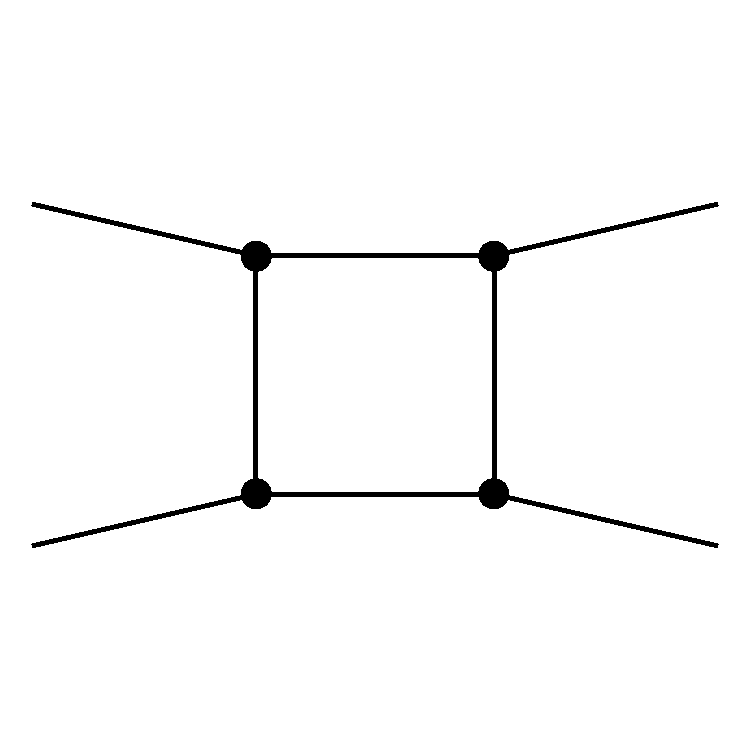
\includegraphics[scale=0.3]{t1}\hspace{-2.4cm}\textbf{T1}\hspace{2.4cm}
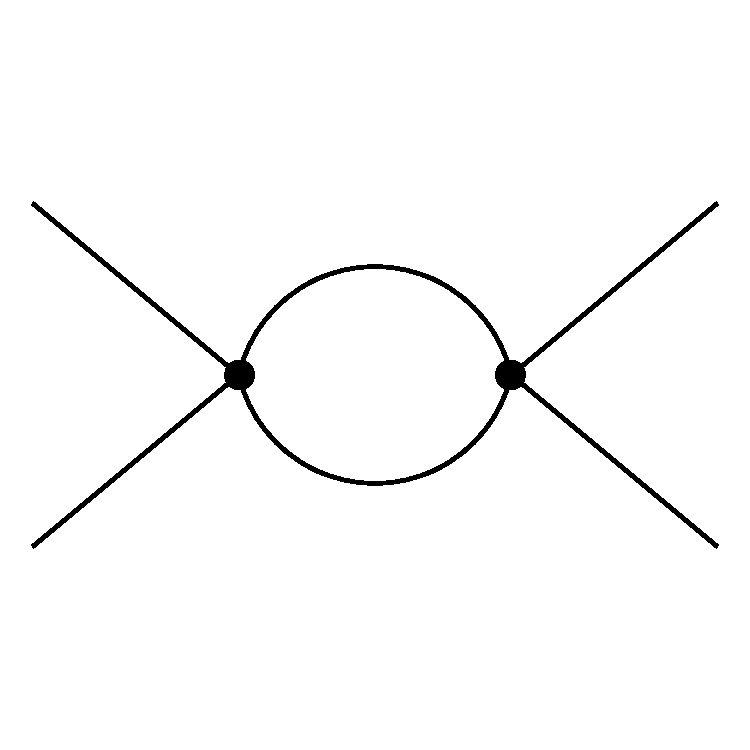
\includegraphics[scale=0.3]{t2}\hspace{-2.4cm}\textbf{T2}\hspace{2.4cm}
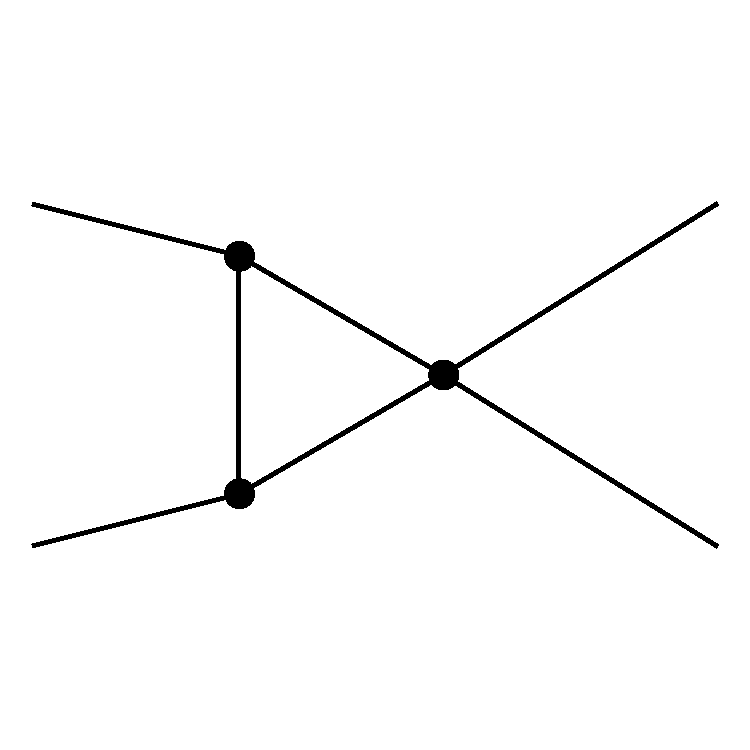
\includegraphics[scale=0.3]{t3}\hspace{-2.4cm}\textbf{T3}\\
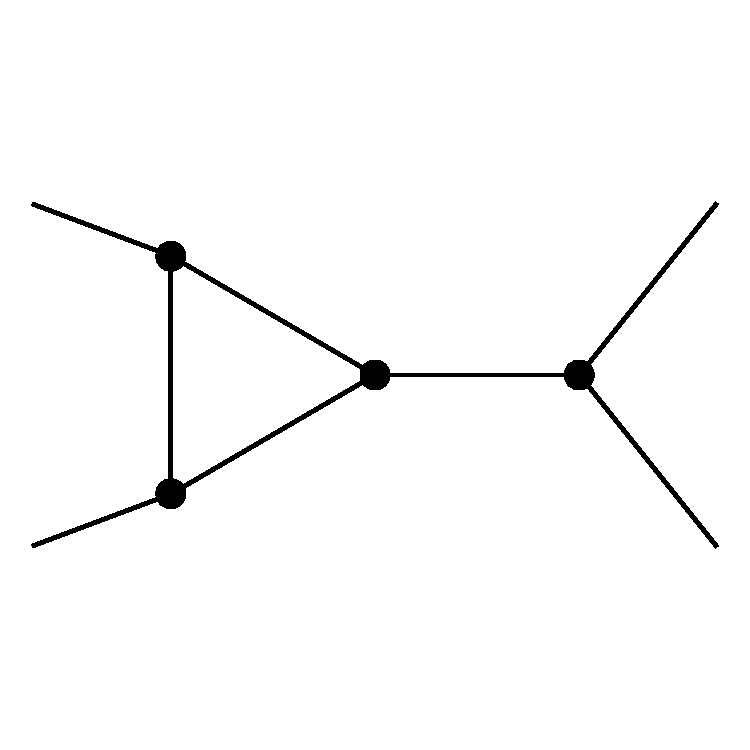
\includegraphics[scale=0.3]{t4}\hspace{-2.4cm}\textbf{T4}\hspace{2.4cm}
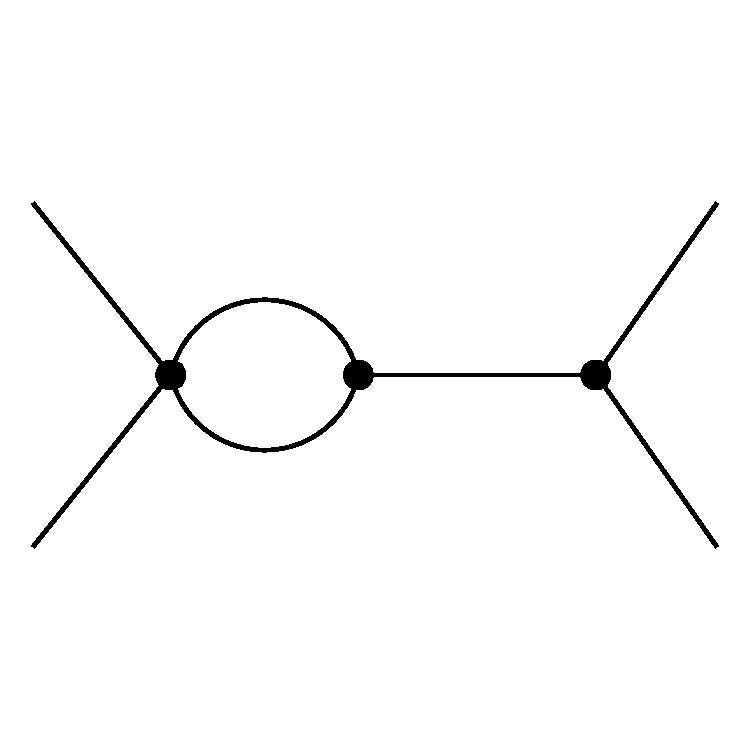
\includegraphics[scale=0.3]{t5}\hspace{-2.4cm}\textbf{T5}\hspace{2.4cm}
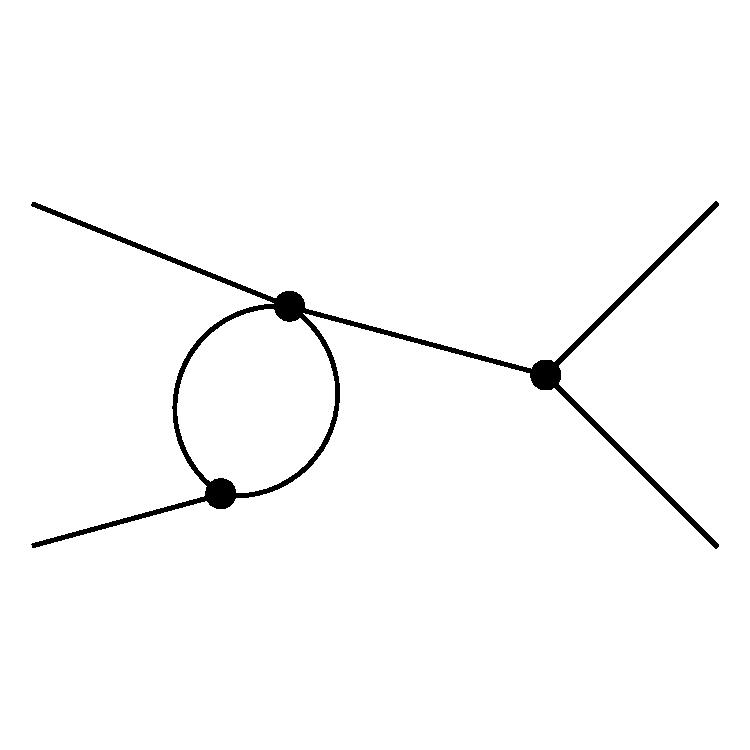
\includegraphics[scale=0.3]{t6}\hspace{-2.4cm}\textbf{T6}
\caption{Topologies of one-loop diagrams with four external legs.}
\label{fig:topologies}
\end{figure}

\begin{table}[h]
\centering
\begin{tabular}{|lccc|}\hline
Particle & {\bf $Z_2$} & {\bf $U(1)_\text{em}$} & Line\\\hline\hline
$\DM$ & -1 & 0 & 
\includegraphics[scale=0.2]{../figures/lineDM} \\
$\DMp(\DM^{\pm})$ & -1 & $1$ & 
\includegraphics[scale=0.2]{../figures/lineDMp} \\
$\medp$ & 1 & $1$ & 
\includegraphics[scale=0.2]{../figures/linephip}\\
$\medz$ & 1 & 0 & 
\includegraphics[scale=0.2]{../figures/linephi0}\\\hline
\end{tabular}
\caption{Generic particle content.}
\label{table:mediators}
\end{table}

Conditions \cond  $\,$allow us to classify all diagrams leading to DM annihilation into photons. Eventually, from this classification, we will write down the interaction Lagrangians that give rise to those processes.  
Let us first notice that condition \hyperref[condition:ii]{(ii)}  implies that DM does not annihilate into two photons at tree level. Moreover, as a consequence of requirement \hyperref[condition:vi]{(vi)}, the corresponding one-loop amplitude  must be finite.  

Notice that every one-loop diagram must take the form of one of the topologies shown in Fig.~\ref{fig:topologies}, which we enumerated for later convenience. From condition \hyperref[condition:i]{(i)}, we also know that each diagram must have  a $Z_2$ line starting and ending at the DM particles in the initial state. Moreover, since conditions \hyperref[condition:ii]{(ii)} and \hyperref[condition:iii]{(iii)} forbid the radiation of photons from neutral particles in the diagrams, the fields running in the loop must have electric charge. This means that in addition to the $Z_2$ line, there is closed line in each  diagram  carrying  electric charge.  

According to condition \hyperref[condition:iv]{(iv)}, the electric charge loop is associated to only one field, which we generically call $\DMp$ if it is charged under the $Z_2$ symmetry or $\medp$ in the opposite case. For the sake of simplicity, we assume that  the electric charge of these fields is equal to the  electron charge, however our discussion can be straightforwardly generalized to an arbitrary charge.  
We would like to remark that even though there must be one of these fields in each diagram, we are not restricting ourselves to this minimal content. In fact,   there could be many of these fields in a  given DM theory. Moreover, as we will see later, some diagrams have neutral particles that are even under the  $Z_2$ symmetry and that we generically call $\medz$.  

All these  fields and their quantum numbers are summarized in Table~\ref{table:mediators}, where we also show how we will represent them in Feynman diagrams. In particular, lines associated to the $Z_2$ symmetry are in cyan, whereas, as usual, those associated to the electric charge have an arrow. 
With this assignments, we just proved that every one-loop diagram have a cyan line with its ends in the DM particles in the initial state as well as a loop carrying an arrow. 

Using this observation, we can take each topology in Fig.~\ref{fig:topologies} and assign  fields to its lines by following the next procedure. First, we consider all the possible permutations of the external legs. Second, we draw the lines carrying the $Z_2$ and the electric charge %$U(1)_\text{em}$ 
quantum numbers. Finally, we discard the diagrams that violate one of the conditions stated above. In particular,  according to the requirements \hyperref[condition:ii]{(ii)} and \hyperref[condition:iii]{(iii)},  we will disregard diagrams whose initial legs radiate photons or have neutral particles directly  coupled to two photons.  Interestingly, this procedure %tells us the nature of the mediators involved in the annihilation process and also 
determines the vertices  between the DM and the mediators involved in the annihilation process.  %In fact, our  goal is to determine the Lagrangian associated to these vertices and then calculate the annihilation amplitude from the corresponding Feynman rules. 
%
\newsavebox{\Ta}
\newsavebox{\Tb}
\newsavebox{\Tc}
\newsavebox{\Lagrangian}
\newsavebox{\schLagrangian}
\newsavebox{\Aform}
\newsavebox{\Lagrangianone}
\newsavebox{\Lagrangiantwothree}




%%%%%%%%%%%%%%%%%%%%%%%%%%%%%%%%%%%%%%%%%%%%%%%%

%T1, T2, T3

%%%%%%%%%%%%%%%%%%%%%%%%%%%%%%%%%%%%%%%%%%%%%%%%%%%
%
%
%\begin{table}[h]
\begin{lrbox}{\Ta}
\centering
\begin{tabular}{|c|c|c|}\hline
{\bf Topology} & {\bf Diagrams}% & {\bf Required fields }
 & {\bf Interactions}\\\hline\hline
\multirow{2}{*}{\raisebox{-\height}{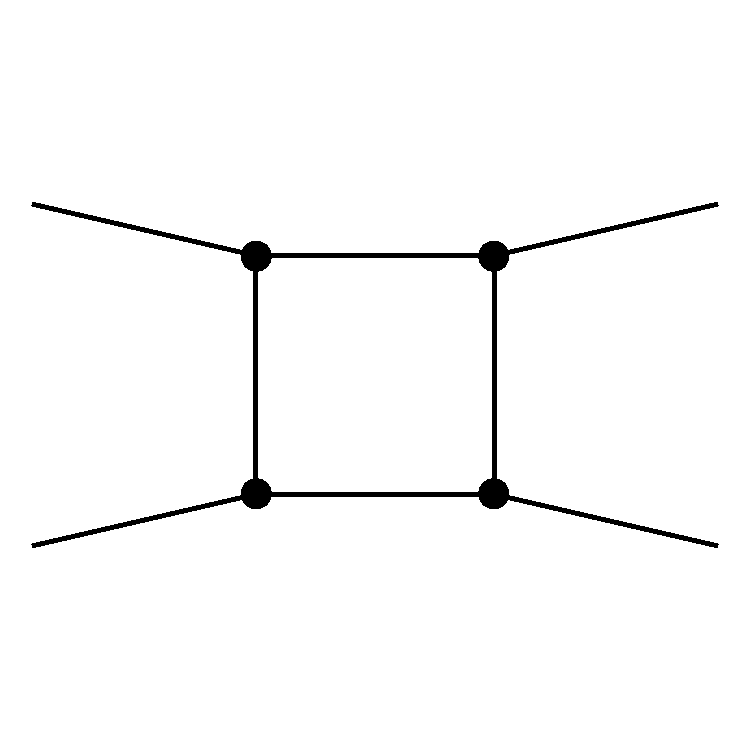
\includegraphics[height=2cm]{t1}}}
&
\raisebox{-.5\height}{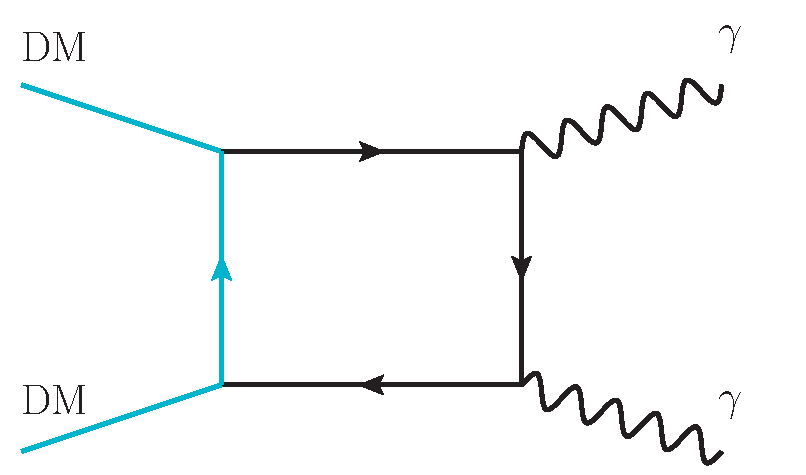
\includegraphics[height=2.3cm]{figures/t1r1}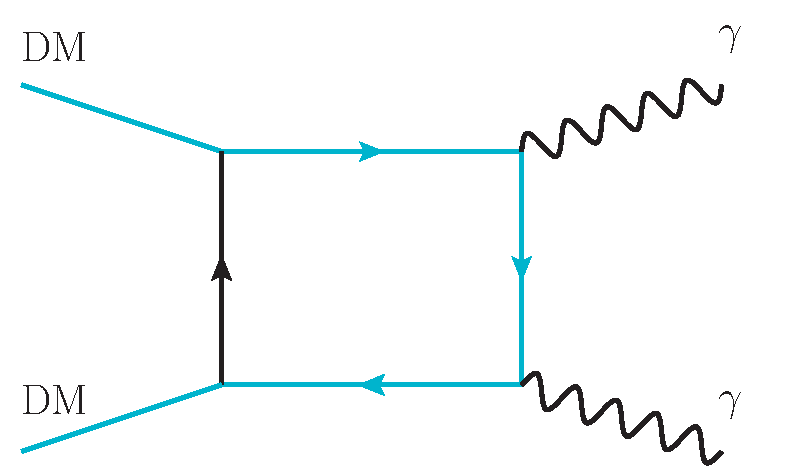
\includegraphics[height=2.3cm]{figures/t1r2}}
%&$\DM, \DM^\pm, \phi^\pm$
&
\dguno

\\\cline{2-3}
T1
&
\raisebox{-.5\height}{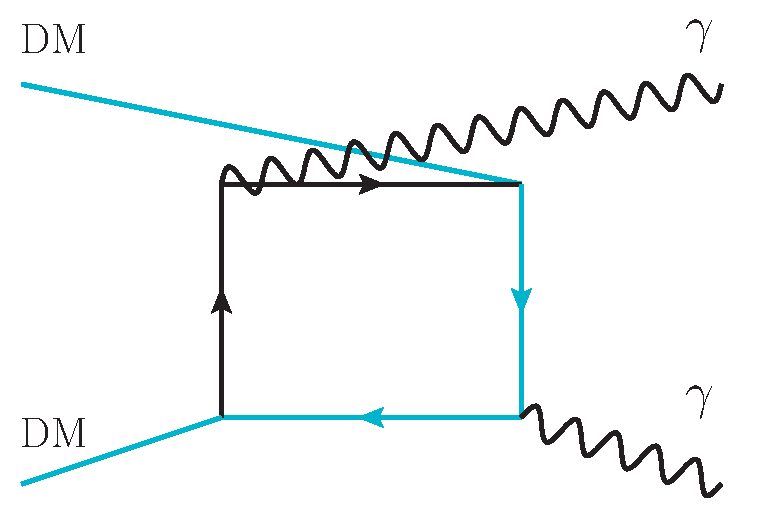
\includegraphics[height=2.3cm]{figures/t1r3}}
%&$\DM, \DM^\pm, \phi^\pm$
&
\dguno

\\\hline
%%%%%%%%%%%%%%%%%%%%%%%%%%%%%%%%%%%%%%%%%%%%%%%
\multirow{2}{*}{\raisebox{-\height}{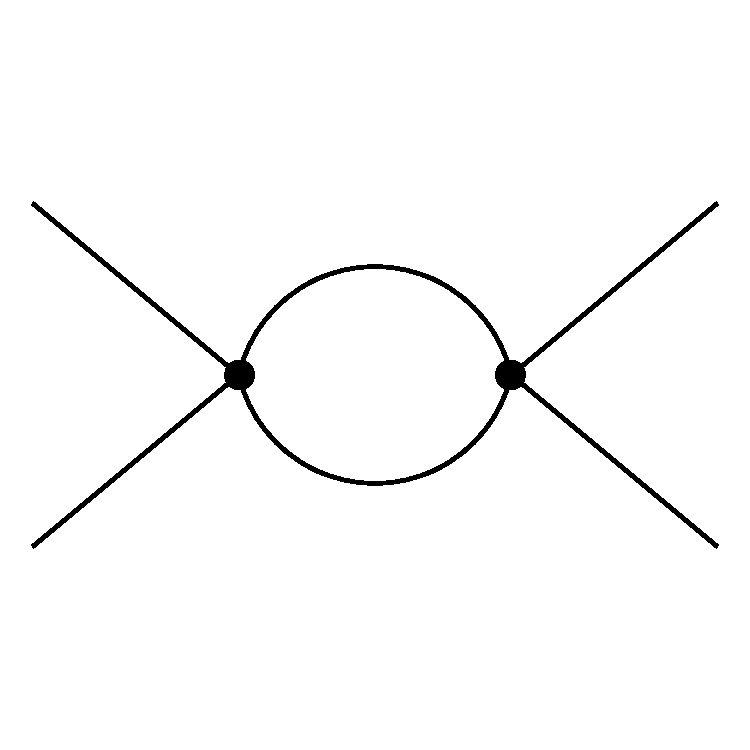
\includegraphics[height=2cm]{t2}}}
&
\raisebox{-.5\height}{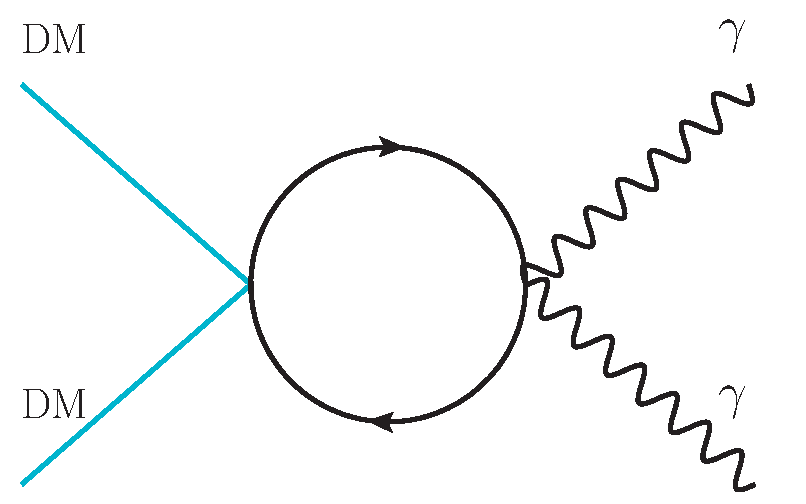
\includegraphics[height=2.3cm]{figures/t2r1}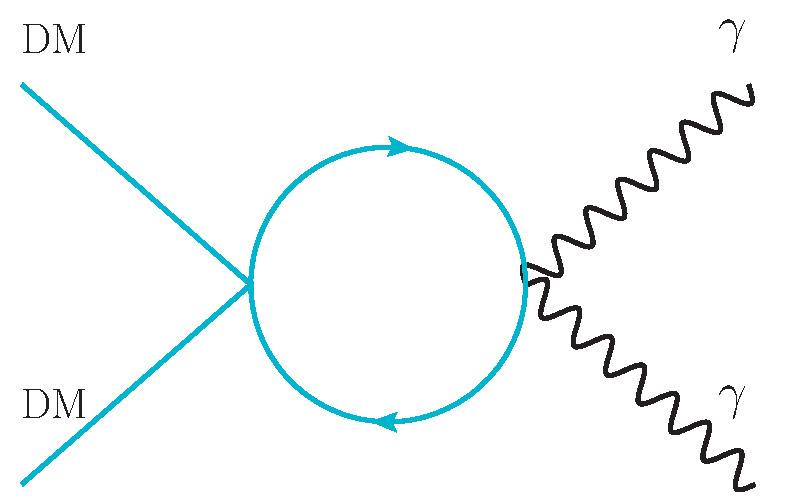
\includegraphics[height=2.3cm]{figures/t2r2}}
%&$\DM, \DM^\pm, \phi^\pm$
&
\dgtres 
\dgdos

\\\cline{2-3}
T2
&
\raisebox{-.5\height}{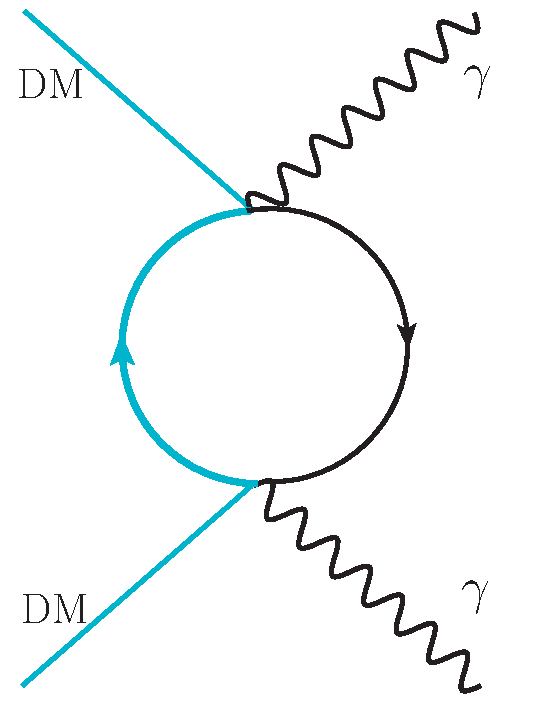
\includegraphics[height=2.3cm]{figures/t2r3}}
%&$\DM, \DM^\pm, \phi^\pm$
&
%\raisebox{-.5\height}{\includegraphics[height=1.5cm]{dg3}}
\dgcuatro

\\\hline
%%%%%%%%%%%%%%%%%%%%%%%%%%%%%%%%%%%%%%%%%%%%%%%
\multirow{3}{*}{\raisebox{-1.5\height}{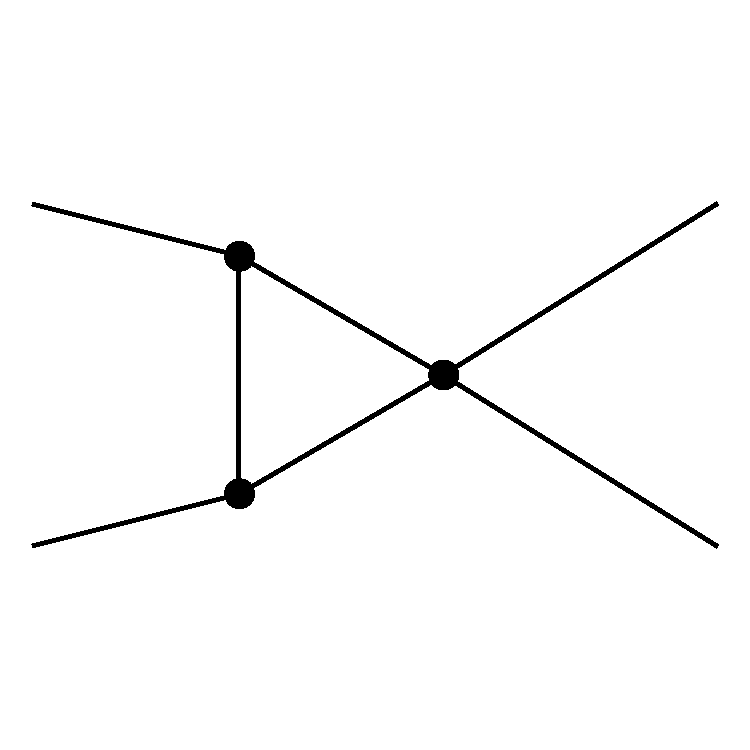
\includegraphics[height=2cm]{t3}}}
&
\raisebox{-.5\height}{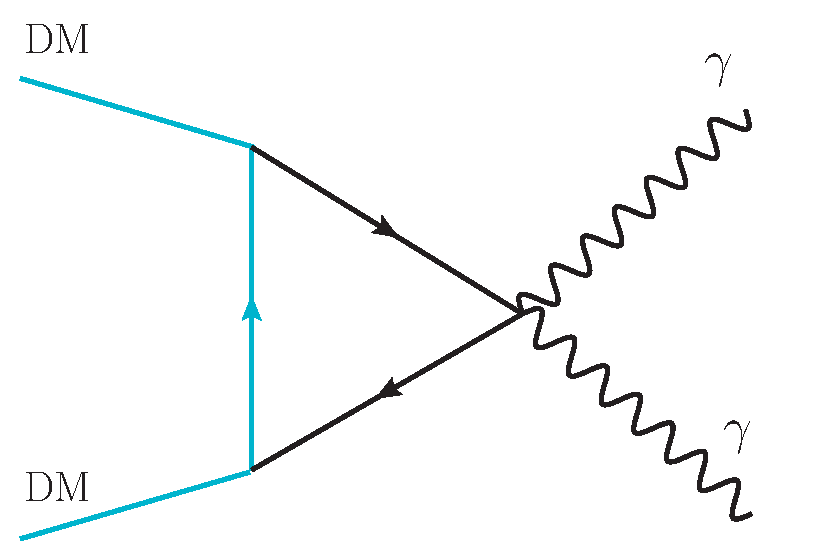
\includegraphics[height=2.3cm]{figures/t3r1}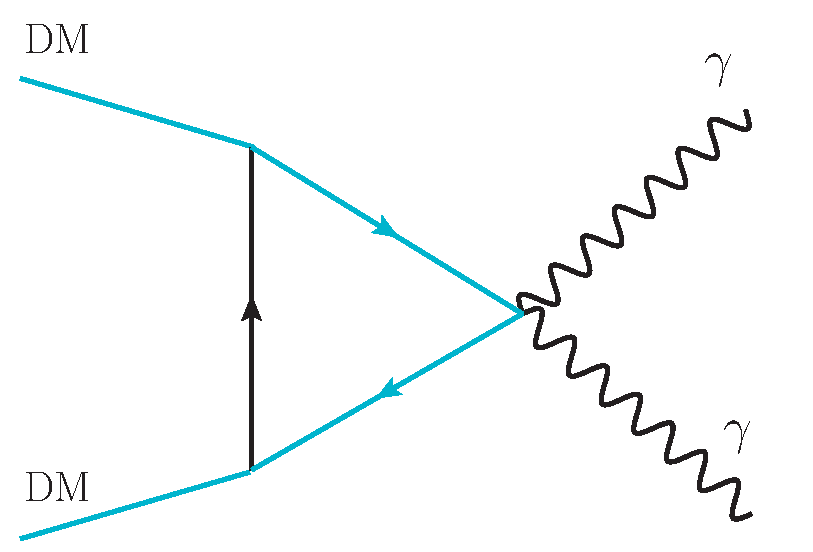
\includegraphics[height=2.3cm]{figures/t3r2}}
%&$\DM, \DM^\pm, \phi^\pm$
&
\dguno

\\\cline{2-3}
&
\raisebox{-.5\height}{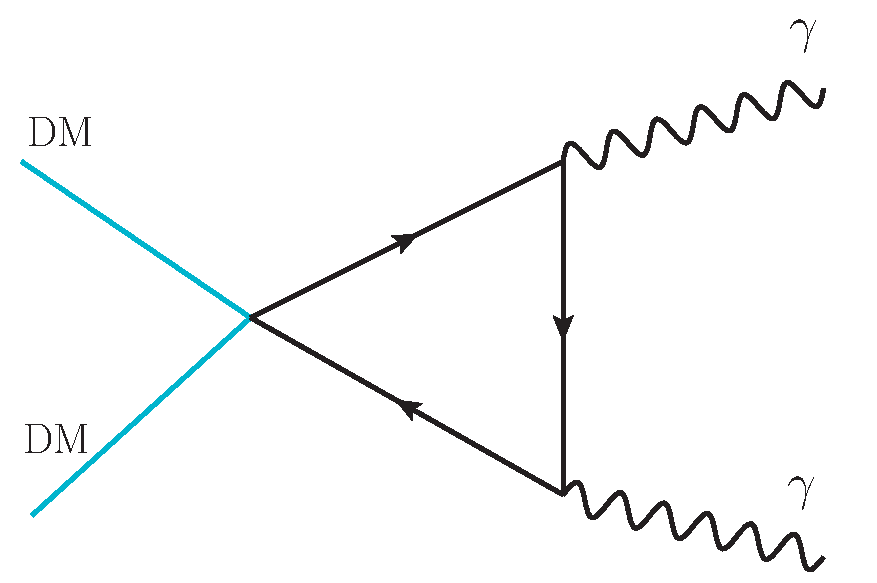
\includegraphics[height=2.3cm]{figures/t3r3}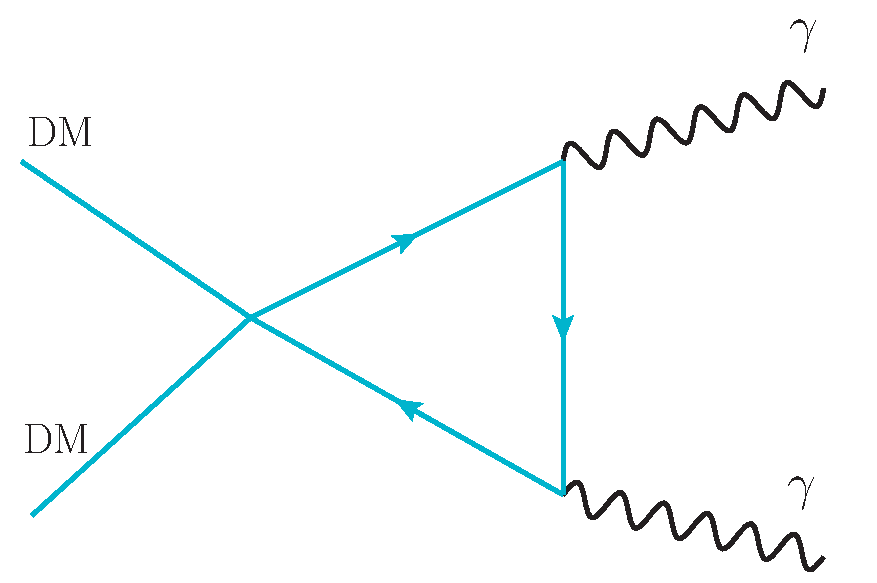
\includegraphics[height=2.3cm]{figures/t3r4}}
%&$\DM, \DM^\pm, \phi^\pm$
&
\dgtres
\dgdos

\\\cline{2-3}
\raisebox{5\height}{T3}
&
\raisebox{-.5\height}{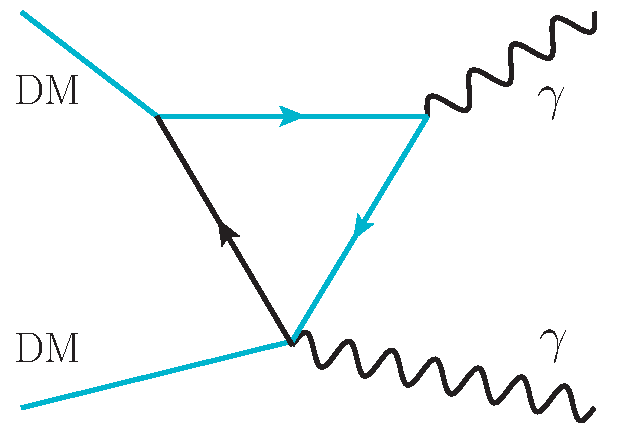
\includegraphics[height=2.3cm]{figures/t3r5}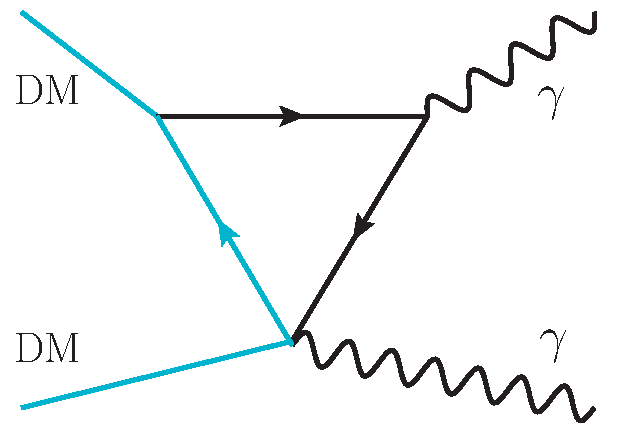
\includegraphics[height=2.3cm]{figures/t3r6}}
%&$\DM, \DM^\pm, \phi^\pm$
&
\dguno
\dgcuatro

\\\hline
\end{tabular}
%\end{table}
%
%
\end{lrbox}






%%%%%%%%%%%%%%%%%%%%%%%%%%%%%%%%%%%%%%%%%%%%%%%%%%%%%%%%%%%%%%%%%%%%%%%%%%

%s-channel: T4 and T5

%%%%%%%%%%%%%%%%%%%%%%%%%%%%%%%%%%%%%%%%%%%%%%%%%%%

\begin{lrbox}{\Tb}
%\begin{table}[h]
\centering
\begin{tabular}{|c|c|c|c|}\hline
{\bf Topology} & {\bf Diagrams} %& {\bf Required fields } 
& {\bf Interactions}\\\hline\hline
\multirow{3}{*}{\raisebox{-1.5\height}{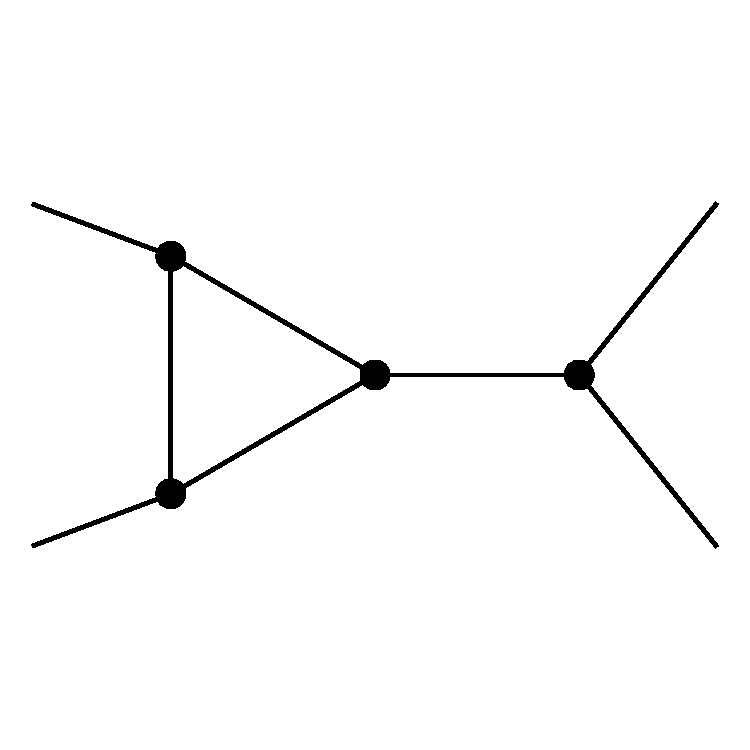
\includegraphics[height=2cm]{t4}}}
&
\raisebox{-.5\height}{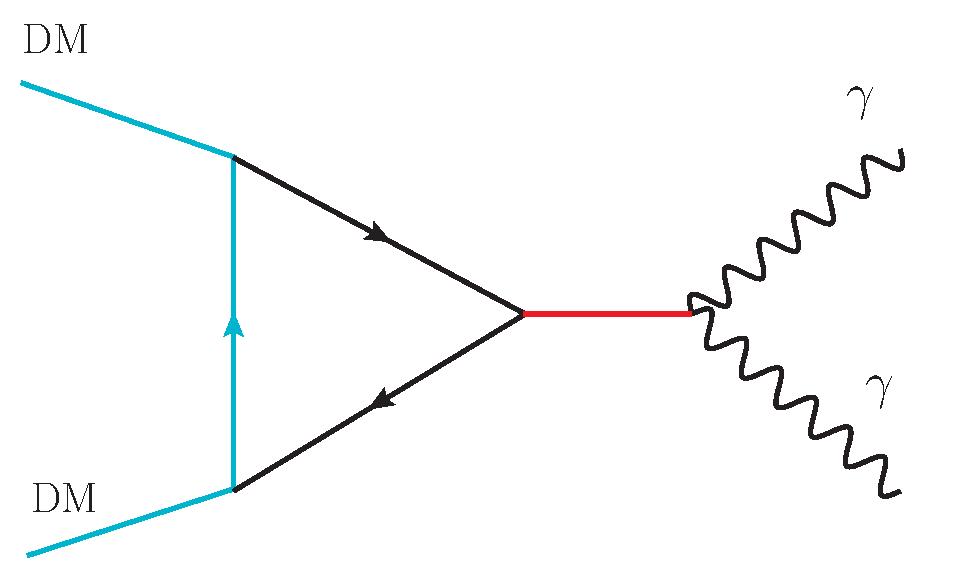
\includegraphics[height=2.3cm]{figures/t4r1}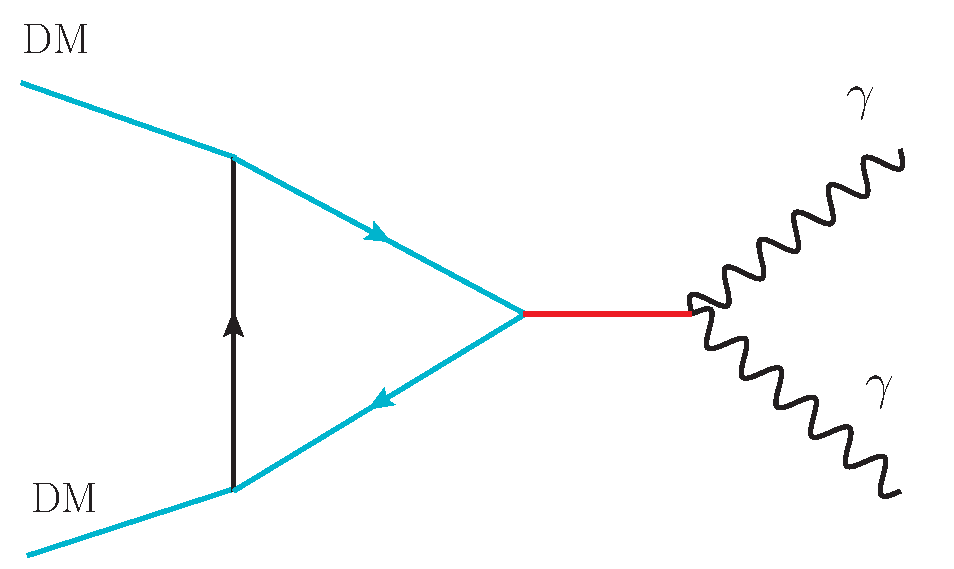
\includegraphics[height=2.3cm]{figures/t4r2}}
%&$\DM, \DM^\pm, \phi^\pm$
&
\Ltwelve

\\\cline{2-3}
&
\raisebox{-.5\height}{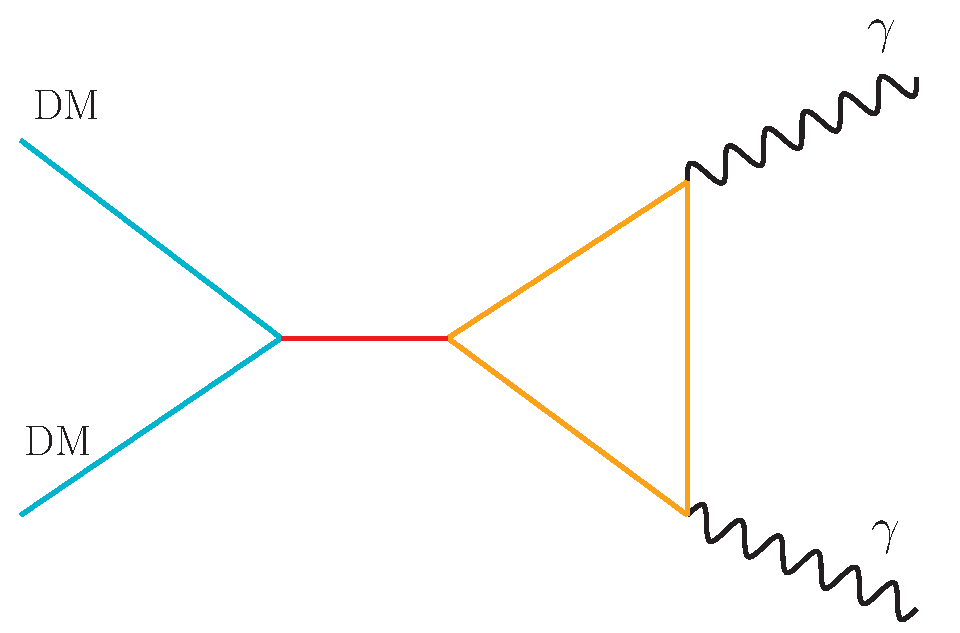
\includegraphics[height=2.3cm]{figures/t4r3}}%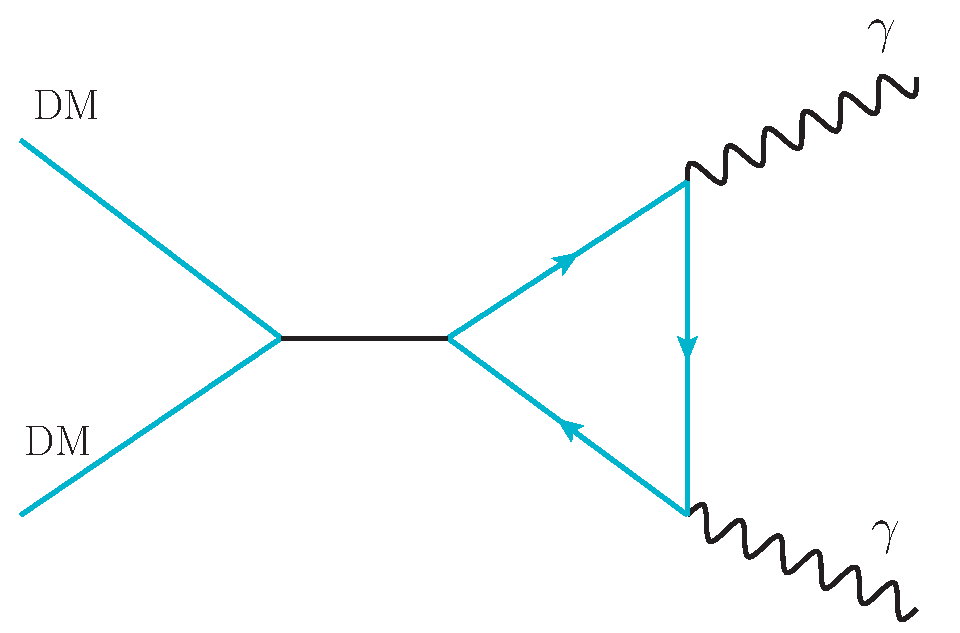
\includegraphics[height=2cm]{figures/t4r4}}
%&$\DM, \DM^\pm, \phi^\pm$
&
\dgcinco \dgseis 
%
\\\cline{2-3}
\raisebox{1.5\height}{T4}
&
\raisebox{-.5\height}{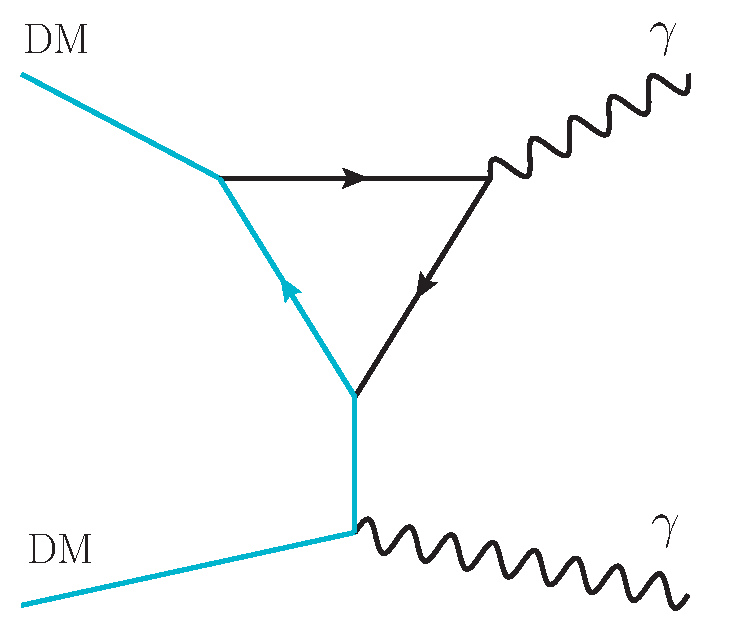
\includegraphics[height=2.3cm]{figures/t4r5}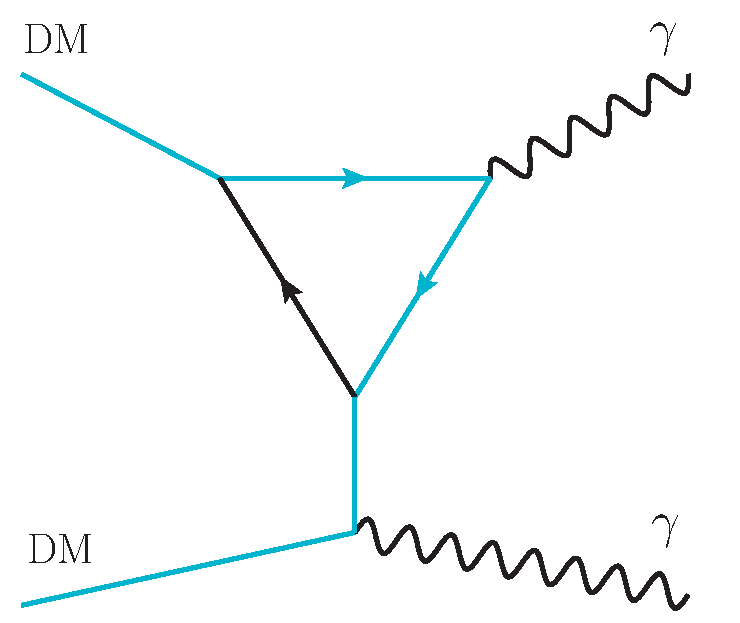
\includegraphics[height=2.3cm]{figures/t4r6}}
%&$\DM, \DM^\pm, \phi^\pm$
&
\Leleven
%
\\\hline
\multirow{3}{*}{\raisebox{-1.5\height}{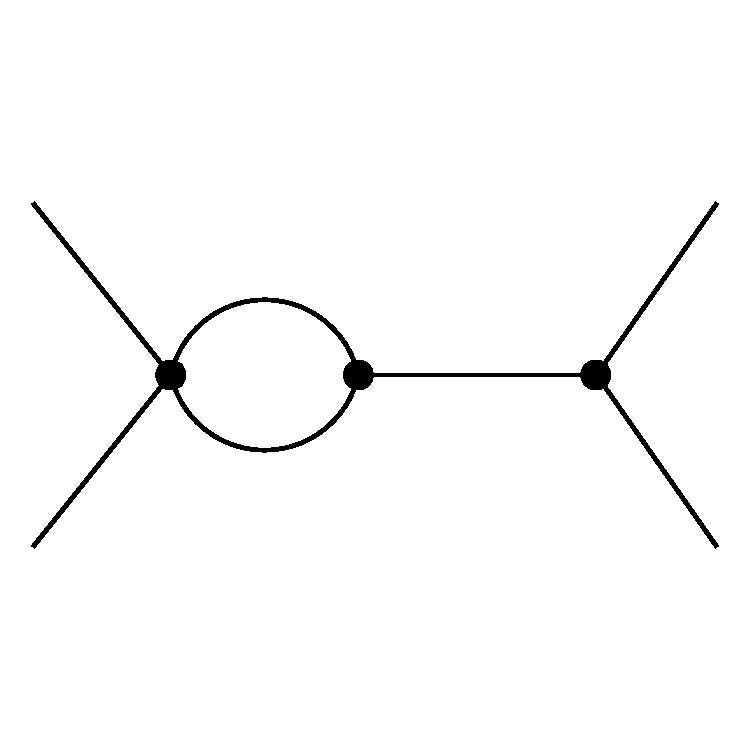
\includegraphics[height=2cm]{t5}}}
&
\raisebox{-.5\height}{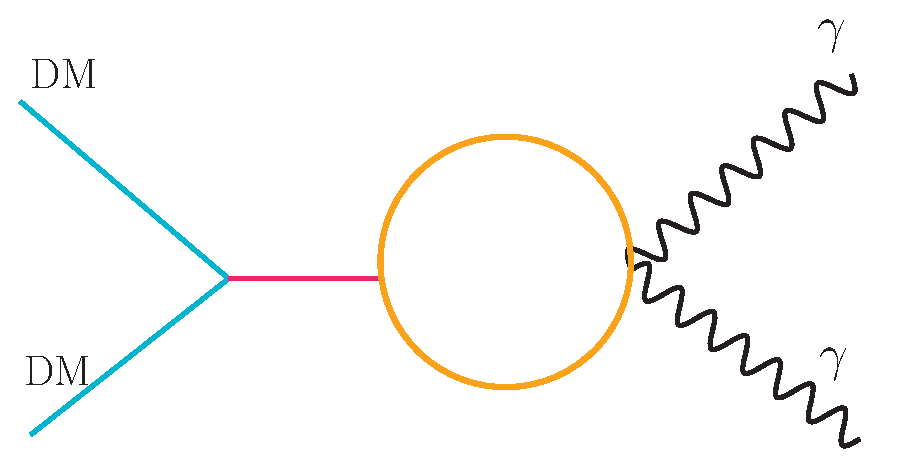
\includegraphics[height=1.7cm]{figures/t5r1}}%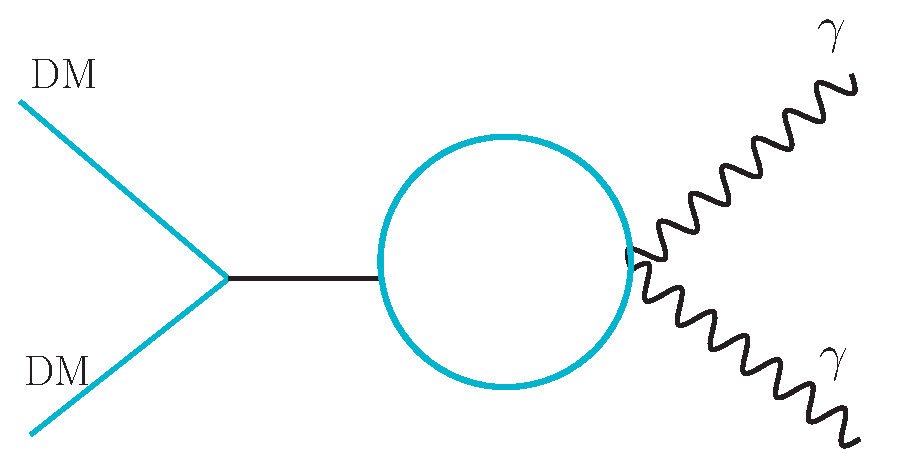
\includegraphics[height=2.3cm]{figures/t5r2}}
%&$\DM, \DM^\pm, \phi^\pm$
&
\dgcinco  \dgseis 

\\\cline{2-3}
&
\raisebox{-.5\height}{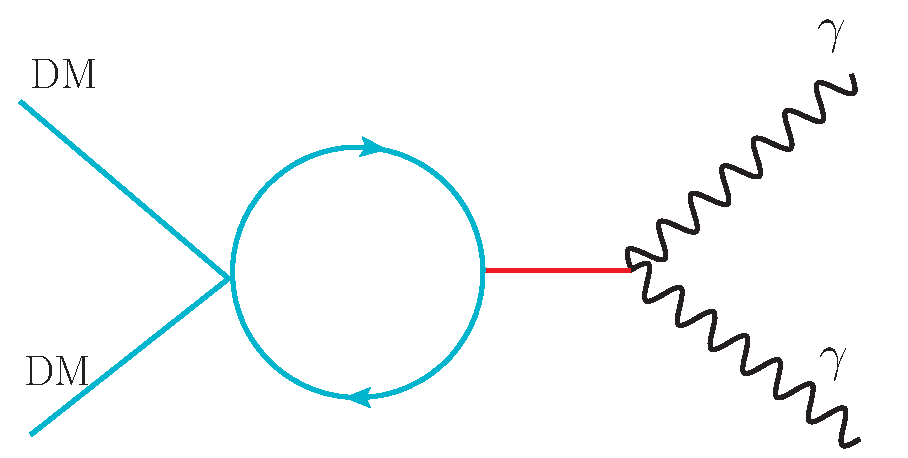
\includegraphics[height=1.7cm]{figures/t5r3}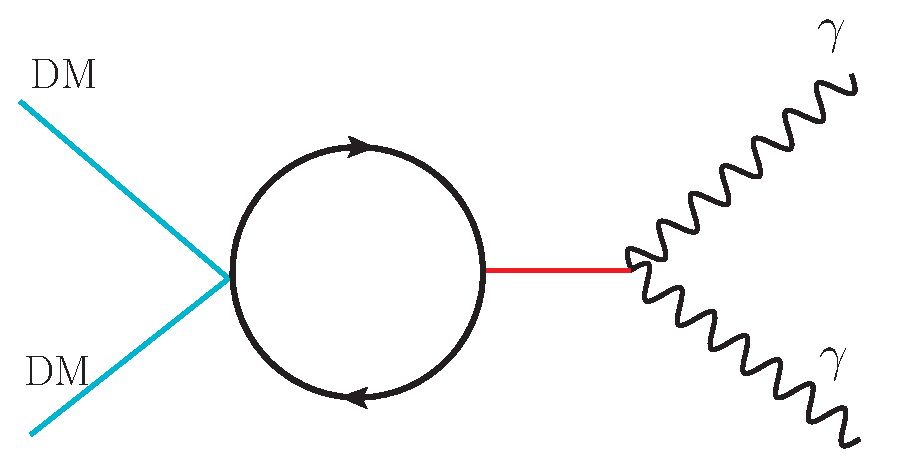
\includegraphics[height=1.7cm]{figures/t5r4}}
%&$\DM, \DM^\pm, \phi^\pm$
&
\Ltwelve

\\\cline{2-3}
\raisebox{5\height}{T5}
&
\raisebox{-.5\height}{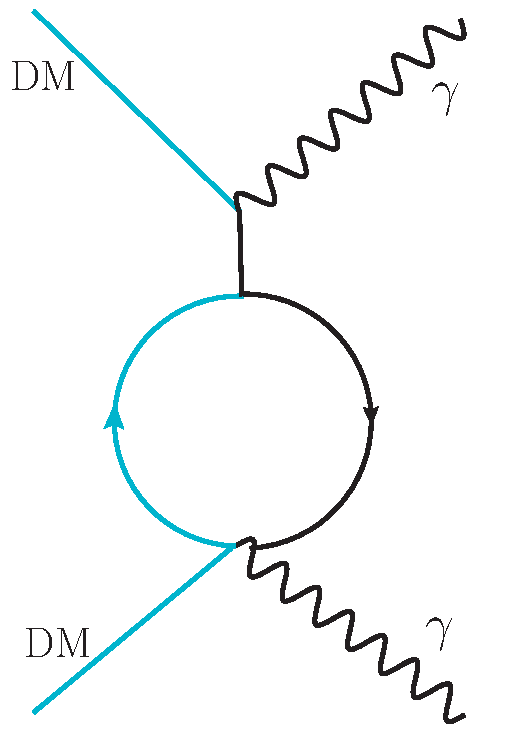
\includegraphics[height=2.9cm]{figures/t5r5}}
%&$\DM, \DM^\pm, \phi^\pm$
&
\Leleven

\\\hline
\end{tabular}
%\end{table}
\end{lrbox}




%%%%%%%%%%%%%%%%%%%%%%%%%%%%%%%%%

% Topology T6

%%%%%%%%%%%%%%%%%%%

\begin{lrbox}{\Tc}
%\begin{table}[h]
\centering
\begin{tabular}{|c|c|c|}\hline
{\bf Topology} & {\bf Diagrams} &% {\bf Required fields } &
 {\bf Interactions}\\\hline\hline
\multirow{4}{*}{\raisebox{-1.7\height}{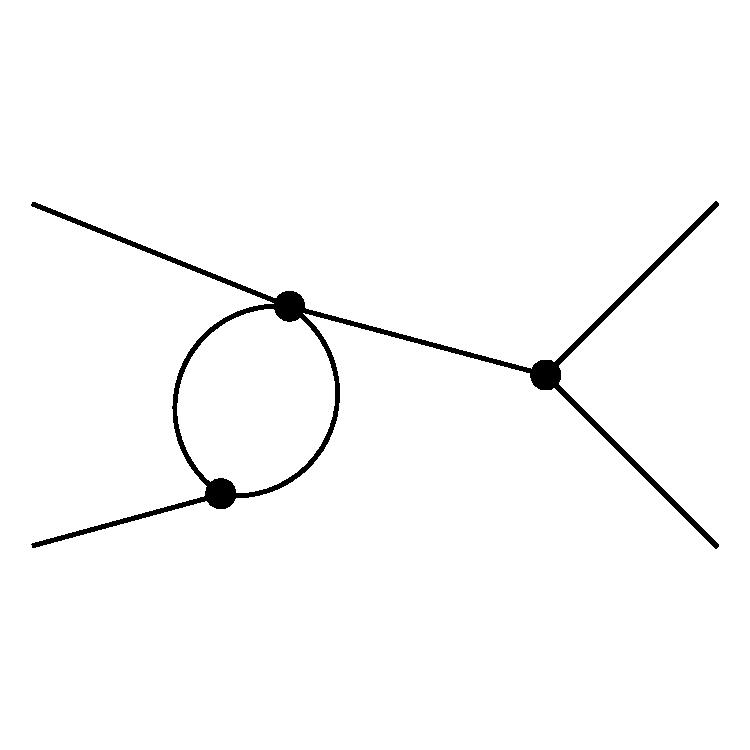
\includegraphics[height=2cm]{t6}}}
&
\raisebox{-.5\height}{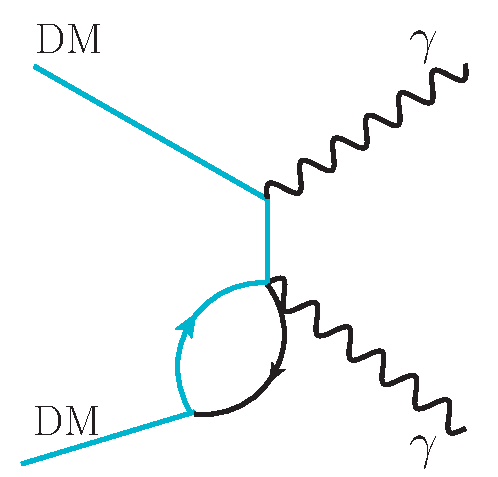
\includegraphics[height=2.3cm]{figures/t6r1}}
&
%$\DM, \DM^\pm, \phi^\pm$&
\Leleven

\\\cline{2-3}
&
\raisebox{-.5\height}{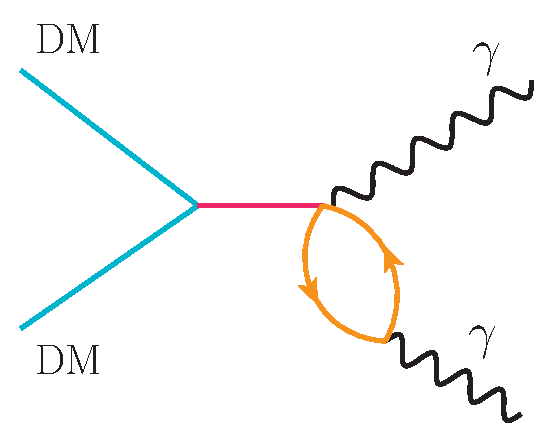
\includegraphics[height=2.3cm]{figures/t6r2}}%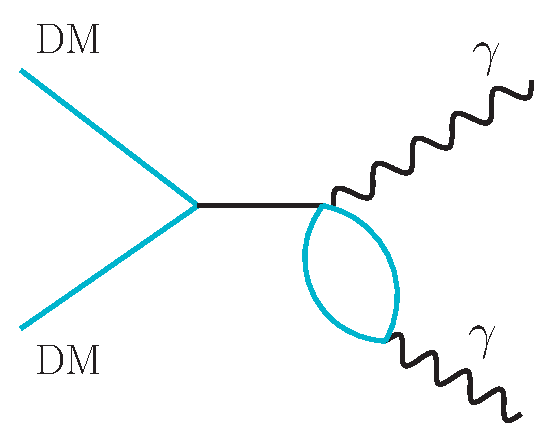
\includegraphics[height=2.3cm]{figures/t6r3}}
&
\dgcinco \dgocho
%$...$
\\\cline{2-3}
T6
&
\raisebox{-.5\height}{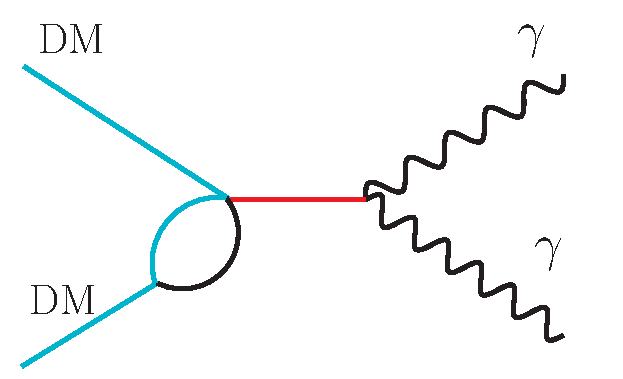
\includegraphics[height=2.3cm]{figures/t6r4}}
&
%$\DM, \DM^\pm, \phi^\pm$&
\Ltwelve 

\\\cline{2-3}
&
\raisebox{-.5\height}{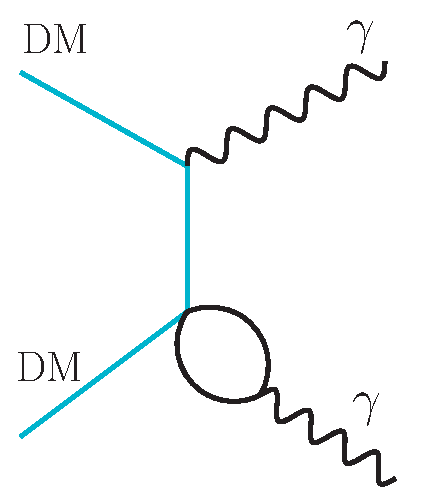
\includegraphics[height=2.3cm]{figures/t6r5}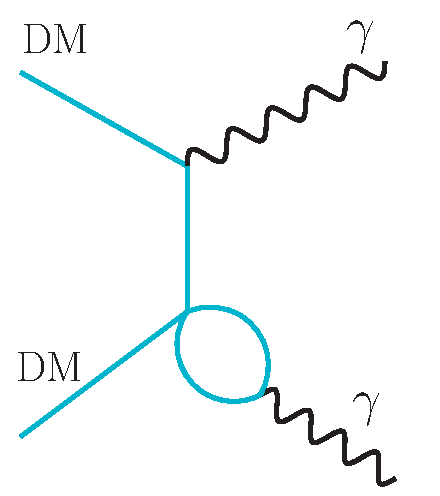
\includegraphics[height=2.3cm]{figures/t6r6}}
&
%$\DM, \DM^\pm, \phi^\pm$&
\Leleven

\\\hline
\end{tabular}
%\end{table}
\end{lrbox}
%%%%%%%%%%%%%%%%%%%%%%%%%%%%%%%%%%%%%%%%%%%%%%%%%%%%%%%%%%%%%%%%%%%%%%%%%%%%%


%%%%%%%%%%%%%%%%%%%%%%%%%%%%%%%%%%%%%%%%%%
%Lagrangian 
%%%%%%%%%%%%%%%%%%%%%%%%%%%%%%%%%%%%%%%%%%%%%
\begin{lrbox}{\Lagrangian}
	\centering
		\begin{tabular}{|c|c|c|c|c|} \hline
%
\multirow{2}{*}{DM field} & \multicolumn{2}{c|}{\multirow{2}{*}{Mediators}}&  \multirow{3}{*}{\dguno}& \multirow{3}{*}{\dgdos\dgtres}\\
\multirow{2}{*}{ $\DM$}&\multicolumn{2}{c|}{}& &
\\\cline{2-3}
 &\,\,$\medp$\,\,\,&$\DMp$&    & \\\hline\hline
\multirow{3}{*}{Real scalar} & S 
 & S
&$g_1\, \DM \, \DMm  \medp  $
&
$\DM^2 \left(g_2\,  \DMp \DMm + g_3\, \medp \medm\right) $
\\\cline{2-5}
&
F & F
&
$
\, \DM\, \overline{\DMp} \left(g_{1L} P_L 
+g_{1R} P_R\right) \medp
$
&
$0$
\\\cline{2-5}
&
V
& S
&$
i  \, {\medp}^\mu\left(g_{11} \DM {\cal D}_\mu  \DMm +g_{12}{\cal D}_\mu \DM\DMm \right)
$
&
$
 \DM^2 (g_2\, \DMp \DMm +g_3\, \medp_\mu {\medm}^\mu )
$
\\\hline
%
\multirow{3}{*}{Majorana}
& S 
& F
& 
$
\medp \overline{\DM} \left(g_{1L} P_L
+g_{1R} \,P_R \right)\DMm 
$
&
\multirow{3}{*}{0}
\\\cline{2-4}
& F
& S
&
$
\DMm\overline{\DM}\left(g_{1L} P_L +g_{1R} P_R \right) \medp 
$
&
\\\cline{2-4}
& V 
& F
&
$
 \overline{\DM}\medp^\mu \gamma_\mu \left( g_{1L} P_L + g_{1R}  P_R \right)\DMm 
$
&
\\\hline
\multirow{2}{*}{Real vector} &
S
 & S
&
$ i g_1  \,\DM^{\mu}  ( {\cal D}_\mu \DMm \medp - \DMm {\cal D}_\mu \medp) $ 
&

$ \DM_\mu \DM^\mu \left(g_2\,  \DMp \DMm+ g_3\, \medm  \medp\right)$
\\\cline{2-5}
&
F & F
&
$
 \overline{\DMp} \DM^{\mu }\gamma_{\mu }  \left( g_{1L} P_L  
+g_{1R}  P_R \right)\medp
$
&
0
\\\hline
\end{tabular}
\end{lrbox}


%%%%%%%%%%%%%%%%%%%%%%%%%%%%%%%%%%%%%%%%%%
%Lagrangian s-channel 
%%%%%%%%%%%%%%%%%%%%%%%%%%%%%%%%%%%%%%%%%%%%%


\begin{lrbox}{\Aform}
	\centering
		\begin{tabular}{|c|c|c|} \hline
%
\multicolumn{2}{|c|}{\multirow{2}{*}{Mediators}}&  \multirow{3}{*}{\dgseis}\\
\multicolumn{2}{|c|}{}&
\\\cline{1-2}
 \,\, $\medz$\,\,\,&\,\,\,\,\,$\medp$\,\,\,\,\,&     \\\hline\hline
\multirow{3}{*}{CP-even}  
 & S
&$g_6 \medz \, \medm \medp   $
\\\cline{2-3}
& F
&
$g_6 \medz \, \overline{\medp} \medp   $
\\\cline{2-3}
&
V
&
$g_6 \medz {\medm}^\mu{\medp}_\mu$
\\\cline{2-3}
&
Gh
&
$g_6 \medz \, \left(\overline{\med}^-\medp+\overline{\med}^+ \medm \right)   $
\\\hline
\multirow{3}{*}{CP-odd}  
 & S
&$0  $
\\\cline{2-3}
& F 
&
$i g_6 \medz \, \overline{\medp}\gamma_5 \medp   $
\\\cline{2-3}
&
V
&
0 
\\\cline{2-3}
&
Gh
&
$ig_6 \medz \, \left(\overline{\med}^-\medp-\overline{\med}^+ \medm \right)   $
\\\hline
\end{tabular}
\end{lrbox}





\begin{lrbox}{\schLagrangian}
	\centering
		\begin{tabular}{|c|c|c|} \hline
%
%
\multirow{3}{*}{DM field $\DM$} & \multirow{3}{*}{ Mediator $\medz$}&  \multirow{3}{*}{\dgcinco}\\
& & 
\\ &&\\\hline\hline
\multirow{2}{*}{Real scalar} & CP-even  
&$g_5 \medz \DM^2$
\\\cline{2-3}
& CP-odd & 0
\\\hline
%
\multirow{2}{*}{Majorana}
& CP-even  
& 
$
g_5\medz \overline{\DM}\DM
$
\\\cline{2-3}
& CP-odd  
& 
$
i g_5\medz \overline{\DM}\gamma_5\DM
$
\\\hline
\multirow{2}{*}{
Real vector
}
&CP-even  
&
$
g_5 \medz \DM_\mu \DM^\mu
$
\\\cline{2-3}
& CP-odd & 0
\\\hline
\end{tabular}
\end{lrbox}



\begin{table}[H]
\usebox{\Ta}
\caption{Topologies 1, 2 and 3.}
\label{table:T123}
\end{table}

To illustrate the previous procedure, let us first discuss  topologies 1, 2 and 3. The corresponding diagrams are in Table~\ref{table:T123}.   
 None of them violates any of our conditions \cond. In fact, they all arise in the one-loop calculation as long as the interaction vertices listed in front exist. These are
%
\begin{align}&
\raisebox{-.5\height}{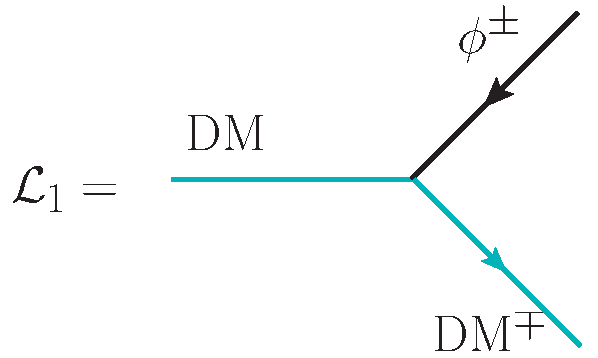
\includegraphics[height=2.0cm]{figures/dg1}}\,, &
\raisebox{-.5\height}{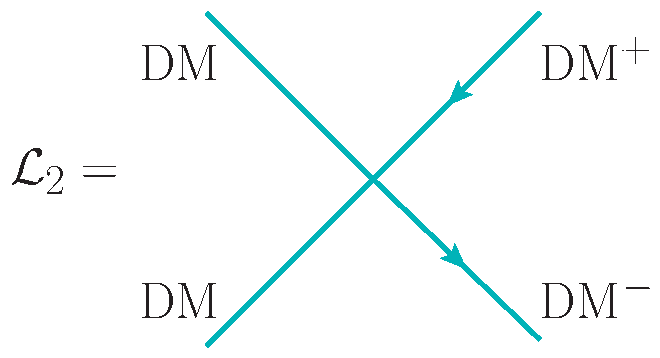
\includegraphics[height=2.0cm]{figures/dg2}}\,, \nonumber\\&
\raisebox{-.5\height}{\includegraphics[height=2.0cm]{figures/dg3}}\,,&
\raisebox{-.5\height}{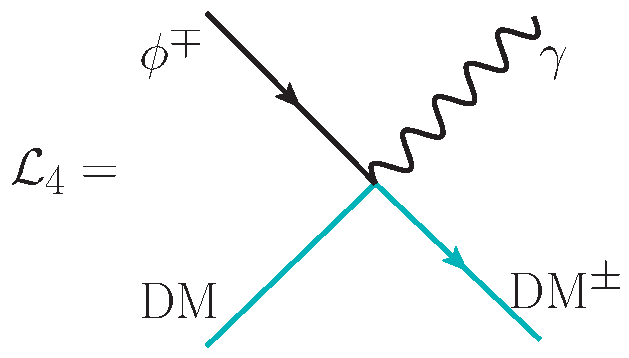
\includegraphics[height=2.0cm]{figures/dg4}}\,.
\label{eq:T123}
\end{align}

%{\color{blue}We will do that in see Sec.~\ref{sec:T345}}

%%%%%%%%%%%% T4 and T5 %%%%%%%%%
\begin{table}[H]
\centering
\usebox{\Tb}
\caption{Topologies 4 and 5.}
\label{table:T45}
\end{table}
%%%%%%%%%%% T6 %%%%%%%%%
\begin{table}[h]
\centering
\usebox{\Tc}
\caption{Topology 6.}
\label{table:T6}
\end{table}

A similar discussion applies to topologies 4, 5 and 6. The corresponding diagrams are shown in Tables ~\ref{table:T45} and ~\ref{table:T6}. In front of each diagram,  we write either the interaction vertices that these diagrams require or if it must be discarded because it violates one of the conditions stated above.  Interestingly, all the viable diagrams that can be constructed out of topologies 4, 5 and 6 correspond to s-channel diagrams involving a neutral particle $\medz$, which couples to the DM at tree-level and that subsequently decays into two photons via a loop of charged particles. Hence,  for these particular topologies, our problem is reduced to calculating the off-shell decay of $\medz$.  We will discuss this more in detail in Sec.~\ref{sec:schannels}. Here, we just mention that for that to be possible  we need the interactions responsible for the production 
 
\begin{align}
\raisebox{-.5\height}{\includegraphics[height=2.6cm]{figures/dg5}}\,,
\label{eq:lscprod}
\end{align}
as well as those associated to the decay
\begin{align}&
\raisebox{-.5\height}{\includegraphics[height=2.5cm]{figures/dg6}} \,,&\raisebox{-.5\height}{\includegraphics[height=2.5cm]{figures/dg8}}\,.
\label{eq:lscdecay}
\end{align}


We arrive to conclusion that, in any DM model satisfying conditions \cond, the annihilation into two photons has an  amplitude  that  can be split into two pieces
\begin{equation}
{\cal B} ={\cal B}\bigg|_{\substack{\text{Topologies}\\\text{1, 2 and 3}}}+{\cal B}\bigg|_\text{s-channel} \,.
\label{eq:Msplit}
\end{equation}  
On the one hand, the first term includes diagrams associated to topologies 1, 2 and 3, which must be calculated by means of the vertices in Eq.~\eqref{eq:T123}. On the other hand,  the second term  is associated to a DM pair exchanging a neutral particle in the s-channel which subsequently decays into photons. Such amplitude requires the vertices in Eq.~\eqref{eq:lscprod} or  Eq.~\eqref{eq:lscdecay}. 


Before closing this section, we would like to remark that
even though the total annihilation amplitude is gauge invariant, that is not necessarily  the case of each piece in Eq.~\eqref{eq:Msplit}. Hence, we have to carefully specify a gauge for our one-loop amplitude. Conditions \cond $ $ also set restrictions on this matter. For fermions or scalars, condition \hyperref[condition:iv]{(iv)} just demands that no FCNC are present. However, for gauge bosons, the situation is more involved because photons could couple to Goldstone and gauge bosons in the same cubic vertex. For instance,  vertices such as $\gamma \,G^+ \,W^-$  are present in linear $R_\xi$ gauges of the SM such as the Feynman gauge (Here, $G^+$ is the Goldstone boson associated to the $W^+$ boson). Nevertheless, as pointed out in Ref.\cite{Bergstrom:1997fh}, in non-linear gauges, condition \hyperref[condition:ii]{(ii)} is satisfied because such vertices are absent~\cite{Fujikawa:1973qs}. We refer the reader to appendix~\ref{sec:Gauge} for a detailed discussion. Here, we just mention that  we  will always work in one of those non-linear gauges.

We can now write down explicitly each of the Lagrangians in Eqs.~\eqref{eq:T123}, \eqref{eq:lscprod} and \eqref{eq:lscdecay}, and calculate the corresponding amplitudes. This is the subject of the following section.










\section{Calculation of the amplitude}
\subsection{Topologies 1, 2 and 3}
\label{sec:T123}

\begin{table}[H]
\usebox{\Lagrangian}
\caption{General interactions.}
\label{table:Lagrangian}
\end{table}

In this section, we calculate the form factors ${\cal B}$ associated to topologies 1, 2 and 3, which lead to the diagrams shown in Table~\ref{table:T123}. To that end, we must specify the spin of both the DM and the mediators, or equivalently, what sort of fields they are, so that we can construct their Lagrangian. %We will be as general as possible. 


Let us start with the DM field.  Condition \hyperref[condition:v]{(v)} implies that DM must be a real scalar, a Majorana fermion or a real vector field. 
With respect to the mediators, we will assume that $\DMp$ is either a complex scalar (S) or a fermionic field (F). Since it is charged under $Z_2$,  we do not consider the possibility of $\DMp$ as a vector boson. Charged spin-1 particles can only be described in a renormalizable way by means of a non-abelian gauge boson, which must not be charged under a $Z_2$ symmetry, as explained above. 

Additionally, we will assume that $\medp$ is a scalar (S), a fermion (F) or a gauge boson (V). Note that Goldstone bosons - which are necessary in the non-linear Feynman gauge- are included in this list. Also, notice that the Padded--Popov ghosts are not considered here because  if they  arose in topologies 1, 2 or 3, DM would directly couple to them, that is, DM would be a gauge boson, a Goldstone particle or a scalar field acquiring a vev; all of which is forbidden by the $Z_2$ symmetry (See Appendix~\ref{sec:Gauge} for more details about  Ghosts in the non-linear gauge). We will see later that ghosts must nevertheless be considered for topologies 4 and 5, which involve s-channel mediators.  We discuss now the interaction Lagrangians.

\subsubsection{Interactions of DM field $\DM$ with  the charged mediators $\DMp$ and $\medp$} 
If we restrict to the previous possibilities, for each of them we can write down the most general Lagrangian associated to the interaction vertices of  Eq.~\eqref{eq:T123}. We show this in Table~\ref{table:Lagrangian}, where the letters S, F and V specify the nature of each field, and stand schematically for scalar , fermionic and vector, respectively. Furthermore, in each case we use generic couplings whose subindex corresponds to the Lagrangian they belong to. Notice that we did not write down the Lagrangians ${\cal L}_4$ of Eq.\eqref{eq:T123}.
This is because gauge invariance demands that these interactions can only arise from the covariant derivative associated to the photon gauge field. 

\begin{comment}
In fact, at it is clear from the table, this only happens for the cases SVS (i.e. scalar DM coupled to a vector field $\medp_\mu$ and scalar DM$^+$) and VSS (vector DM coupled to only scalars). The corresponding Lagrangians are  
%
\begin{align}
{\cal L}_4^{(\text{SVS})} = - ie\,\left(g^{\tiny (1)}_1 +g^{\tiny (2)}_1\right) \text{DM} {\medp}^\mu  \text{DM}^- A_\mu   
+h.c.
%
\\ 
{\cal L}_4^{(\text{VSS})} = - ie\,  \left( g^{\tiny (1)}_{1}+ g^{\tiny (2)}_{1}\right)   \text{DM}^{\mu}\,\medp \text{DM}^-  A_\mu 
+
h.c.
\label{eq:L4}
\end{align}
\CG{Check this!!}
%
\end{comment}
\subsubsection{Interactions of the charged mediators $\DMp$ and $\medp$ with  photons}  
For scalar and fermions, that is trivial as they are described by the usual expressions

\begin{align}
{\cal L}_{\substack{Scalar\\Mediators}} &=  {\cal D}_\mu \medm  {\cal D}^\mu \medp + 
 {\cal D}_\mu \DMm  {\cal D}^\mu \DMp - \mmed^2\, \medm \medp -\mDMp^2\, \DMm \DMp \,,\label{eq:ScalarMediator}
\\
{\cal L}_{\substack{Fermionic\\Mediators}} &=i\overline{\medp}  \slashed{\cal D}\medp +
 i\overline{\DMp}  \slashed{\cal D}\DMp - \mmed\, \overline{\medp} \medp- \mDMp\, \overline{\DMp} \DMp\,. \label{eq:FermionicMediator}
\end{align}
%
where ${\cal D}= \partial - ie A$ is the electromagnetic covariant derivative and $A$ is the photon field. 
The case of the vector mediators $\medp^\mu$ is more complicated. As mentioned above, they must be described by a massive gauge field. Hence, a general approach here is not possible because different gauge groups might lead to different charged vector boson interactions. For concreteness, from now on we will assume that the vector mediator reassembles the $W^+$ boson of the SM. This assumption is not so restrictive as it allows to study DM  with electroweak quantum number as well as other  scenarios where DM interacts with other gauge bosons arising from larger gauge symmetries  such as $W'$ bosons in left-right symmetric theories (See e.g. Ref.~\cite{Heeck:2015qra,Garcia-Cely:2015quu}) or 3-3-1 scenarios (See e.g. Ref.~\cite{TavaresVelasco:2001vb}). Therefore, the vector boson Lagrangian is given by 
\begin{equation}
{\cal L }_{\substack{Vector\\Mediator}}=-\frac{1}{2}\left({\cal D}_\mu \medm_\nu -{\cal D}_\nu \medm_\mu \right)\left({\cal D}^\mu \medp^{\nu} -{\cal D}^\nu \medp^{\mu} \right)+ \mmed^2\, \medm^{\mu}\medp_\mu-ie\,F^{\mu\nu} \medp_\mu\medm_\nu +\delta{\cal L}\, .
\label{eq:VectorMediator}
\end{equation}
where $F$ is the electromagnetic field strength and $\delta{\cal L}$ is the piece of the interaction obtained by the gauge-fixing  procedure in the Feynman non-linear gauge (see Appendix~\ref{sec:Gauge} for details)
\begin{equation}
\delta {\cal L}= 
 - e^2 A^\mu A^\nu  \medm_\mu \medp_\nu
+i  e A^\mu ( \medp_\mu \partial^\nu \medm_\nu-  \medm_\mu \partial^\nu \medp_\nu)\,.
\end{equation}
%
%Notice that, in contrast to the scalar and fermionic case, the interactions of the vector mediator with photons are not uniquely determined by electromagnetic gauge invariance.\footnote{The second term in Eq.~\eqref{eq:VectorMediator} arises in the SM from the $SU(2)$ structure of the electroweak interactions. Even though electromagnetic gauge invariance does not restrict the corresponding coupling for an arbitrary charged vector boson, it has been shown that deviations from the value in Eq.~\eqref{eq:VectorMediator} leads to problems with unitarity~\cite{Ferrara:1992yc}.}


Massive vector fields  come with Goldstone bosons and ghosts. While the latter are not relevant for topologies 1, 2 and 3, the former must be taken into account here. If we were to perform the calculation in any of the usual $R_\xi$ gauges, we would have to also introduce interactions between the Goldstone bosons, the charged vector fields and the photons. Nevertheless, the Goldstone bosons decouple from the gauge field  in the non-linear gauge and therefore in that case the relevant piece of their Lagrangian for our purposes  is simply given by Eq.~\eqref{eq:ScalarMediator} (with $\medp$ as the Goldstone boson).  
 
We are now ready  to calculate the ${\cal B}$ factors  for each scenario of Table~\ref{table:Lagrangian}. To that end, by means of \textsc{FeynRules}~\cite{Christensen:2008py,Alloul:2013bka},  we implement the Lagrangians quoted in this table as well as  those of Eqs.~\eqref{eq:ScalarMediator},\eqref{eq:FermionicMediator} and \eqref{eq:VectorMediator} in \textsc{FeynArts}~\cite{Hahn:2000kx} and \textsc{FormCalc}~\cite{Hahn:1998yk}. Then, we calculate the amplitude for the process DMDM$\to\gamma\gamma$ in each case and have \textsc{FormCalc} to reduce their tensor integrals to scalar Passarino-Veltman functions.
%%%% PONER REFERECIA
% {\color{blue}(See e.g. for a review on this procedure, see e.g. )}. 

Unfortunately, for relative DM velocities approaching zero, i.e. $v\to0$, the previous algorithm for reducing the  tensor integrals in the amplitude to scalar functions leads to numerical inestabilities and even breaks down for $v=0$. This pathological behavior is well-understood and stems from the assumption that the external momenta in the annihilation process are linearly independent. Following~\cite{STUART1988367}, we reduce the integrals dropping such assumption. For a detailed description of this procedure, we refer the reader to Appendix~\ref{sec:CD-reduction}.
%%% MY FINAL TEXT 
Specifically, this algorithm reduces the four-point function to three-point functions. Later, we used the \textsc{Package-X}~\cite{Patel:2015tea} to reduce all the remaining coefficients tensor $C_{\mu},C_{\mu\nu},C_{\mu\nu\rho}, \cdots $, to the scalar Passarino Veltman $C_0$~\cite{Passarino:1978jh}. Usually, the results are given in terms of $C_0$ which can be given in terms of the dilogarithm Li$_{2}$ functions. However, in the case of $C_0$, the notation is more compact and readable.

In Sec.~\ref{sec:cond}, based on general considerations such as Lorentz and gauge invariance, we argued that the annihilation amplitude can be cast as shown in Eqs.~\eqref{eq:Mscalar}, \eqref{eq:MMaj} and \eqref{eq:Mvec}. Using the previous procedure, we explicitly  corroborate  that. Furthermore, for a given set of interactions ${\cal L}_1$, ${\cal L}_2$ and ${\cal L}_3$, we can decompose each form factor in terms of Passarino-Veltman functions of two and three points describe in the Appendix~\ref{sec:passarino-veltman}. Concretely,

\begin{align}
%\label{eq:passarino-components}
{\cal B}\bigg|_{\substack{\text{Topologies}\\\text{1, 2 and 3}}}= \dfrac{\alpha}{\pi}\bigg[% {\color{red}\dfrac{x_1}{3(\rmed^2-\rDMp^2+1)}
&x_1 
+x_2 \dfrac{ \, C_0( 0, 1, -1, \rmed ^2, \rmed ^2, \rDMp^2)  }{(\rDMp^2-\rmed^2)(1+\rDMp^2-\rmed^2)}
+x_3 \dfrac{ \, C_0( 0, 1, -1, \rDMp^2, \rDMp^2, \rmed ^2)}{\left(-\rDMp^2+\rmed^2\right)\left(1-\rDMp^2+\rmed^2\right)}\nonumber\\
&+x_4 \,\, C_0\left( 0, 4 \, , 0, \rmed ^2, \rmed ^2, \rmed ^2\right)
+ x_5 \,\,  C_0\left( 0, 4 \, , 0, \rDMp^2,\rDMp^2, \rDMp^2 \right)\nonumber\\
&+x_6\, \left(B_0(4 , \rmed^2 ,\rmed^2 )- B_0(1 ,\rDMp^2, \rmed^2 )\right)\nonumber\\
&+x_7\, \left(B_0(4 , \rDMp^2,\rDMp^2)- B_0(1 ,\rDMp^2, \rmed^2 )\right)\nonumber\\
&+x_8\, \left(B_0(-1 , \rDMp^2,\rmed^2 )- B_0( 1,\rDMp^2, \rmed^2 )\right)%
%-(x_6+x_7)\, B_0( , \rmed ,\rDMp)
\bigg]\,,%\nonumber
\label{eq:B123expansion}
\end{align}

\begin{comment}
\begin{align}
%\label{eq:passarino-components}
{\cal B}_\text{T123}= \dfrac{\alpha}{\pi}\bigg[% {\color{red}\dfrac{x_1}{3(\rmed^2-\rDMp^2+1)}
&x_1 
+x_2 \dfrac{ \mDM^2\, C_0( 0, \mDM^2, -\mDM^2, \mmed^2, \mmed^2, \mDMp^2)  }{(\rDMp^2-\rmed^2)(1+\rDMp^2-\rmed^2)}
+x_3 \dfrac{ \mDM^2\, C_0( 0, \mDM^2, -\mDM^2, \mDMp^2, \mDMp^2, \mmed^2)}{\left(-\rDMp^2+\rmed^2\right)\left(1-\rDMp^2+\rmed^2\right)}\nonumber\\
&+x_4 \,\mDM^2\, C_0\left( 0, 4 \, \mDM^2, 0, \mmed^2, \mmed^2, \mmed^2\right)
+ x_5 \,\mDM^2\,  C_0\left( 0, 4 \, \mDM^2, 0, \mDMp^2,\mDMp^2, \mDMp^2 \right)\nonumber\\
&+x_6\, \left(B_0(4 \mDM^2, \mmed,\mmed)- B_0( \mDM^2,\mDMp, \mmed)\right)\nonumber\\
&+x_7\, \left(B_0(4 \mDM^2, \mDMp,\mDMp)- B_0( \mDM^2,\mDMp, \mmed)\right)\nonumber\\
&+x_8\, \left(B_0(- \mDM^2, \mDMp,\mmed)- B_0( \mDM^2,\mDMp, \mmed)\right)%
%-(x_6+x_7)\, B_0( \mDM^2, \mmed,\mDMp)
\bigg]\,,%\nonumber
\label{eq:B123expansion}
\end{align}
\end{comment}
%
where $\rmed \equiv \mmed/\mDM$, $\rDMp \equiv \mDMp/\mDM$  and $x_i$ are dimensionless coefficients for different combinations of mediators. The same expression holds for $\mathcal{B}_1$, $\mathcal{B}_2$ and $\mathcal{B}_6$ in the case of vector DM.
The goal of this work is to compute all the $x_i$ coefficients for each model (work in process). In this thesis, as an illustration, we only will apply this schema to two particular examples in the Sec.~\ref{sec:two-examples}.











\subsection{Topologies associated to s-channels }
\label{sec:schannels}

\begin{table}[H]
\begin{centering}
\begin{minipage}{0.44\textwidth}
\usebox{\schLagrangian}
\caption{Interactions of $\DM$ with neutral mediators.}
\label{table:schLagrangian}
\end{minipage}
\hspace{40pt}
\begin{minipage}{0.44\textwidth}
\usebox{\Aform}
\caption{Interaction among neutral and charge mediators.}
\label{table:Acal}
\end{minipage}
\end{centering}
\end{table}

As for previous topologies, we must first specify the nature of the particles involved in the annihilation diagram. Tables~\ref{table:T45} and \ref{table:T6} clearly show that the particle in the s-channel is a boson  electrically neutral and even under the $Z_2$ symmetry. 
In Appendix~\ref{sec:Gauge}, we prove that if the particle on the s-channel is a massive gauge boson, its contribution to the annihilation vanishes in the Landau gauge, and only the corresponding  (massless) Goldstone boson must be taken into account. Thus, without loss of generality, we will only consider the possibility of a scalar particle on the s-channel. Furthermore, because we are assuming that CP is conserved, we can classify the the possible s-channel diagrams according to the CP-parity of the scalar mediator.

Using this,  we divide the problem in two parts. On the one hand, we describe how the DM couples to the neutral mediator. This information is carried by the Lagrangian ${\cal L}_5$ of Eq.~\eqref{eq:lscprod}, which we write in  Table~\ref{table:schLagrangian} for each type of DM.  On the other  hand, we describe the off-shell decay of the mediator.  This is done by means of the Lagrangian ${\cal L}_6$ of Eq.\eqref{eq:lscdecay}, which we specify in Table~\ref{table:Acal} for all the possible charged mediators.  Notice that ${\cal L}_7$ vanishes\footnote{This only true if we demand that the charged particles in ${\cal L}_7$ belong to the same field. We do that because we want to satisfy condition~\hyperref[condition:iv]{(iv)} for closing the loop. If we drop this requirement, ${\cal L}_7$ does not vanish. For instance, if the particle in the s-channel is the Higgs boson, vertices such as $h W^+G^-\gamma $ would contribute to the annihilation into photons because the vertex $W^+G^- \gamma$ exists in general (for clearer picture, see the second row of Table~\ref{table:T6}). As discussed previously, in order to avoid these situations, we work in the non-linear Feynman gauge where the latter vertex does not exist.}. In contrast to case of topologies 1, 2 or 3, here we do need to take into account the presence of Ghosts because a scalar particle can interact with them if it also couples to charged gauge bosons. Notice that for each charged gauge boson, there are two  Ghosts, as shown in the Table.  

Combining the information on Tables~\ref{table:schLagrangian} and \ref{table:Acal}, we can calculate the annihilation amplitude for any s-channel process. 
%In analogy to Eq.~\eqref{eq:B123expansion}, for each set ${\cal L}_5$ and ${\cal L}_6$, we find
%
%\begin{align}
%{\cal B}\bigg|_\text{s-channel}= \dfrac{\alpha}{\pi}\bigg[
%&x_9 
%+x_{10}\, C_0\left( 0, 4 , 0, r_{\medp}^2,  r_{\medp}^2,  r_{\medp}^2\right)
%\bigg]\,.%\nonumber
%\label{eq:Bschexpansion}
%\end{align}
%%The coefficients for each case listed in the tables  are found in Appendix~\ref{sec:xs}. 
%
% Before finalizing this section,  w
We discuss the case the Higgs and the $Z$ boson as s-channel mediators. They are very important not only because they arise in many DM models but also because we know their couplings to SM particles and consequently their contribution to the annihilation amplitudes can be calculated precisely.
\begin{itemize}
\item $\medz$ as the Higgs boson. If SM scalar doublet is given by
\begin{equation}
H = \begin{pmatrix} G^+ \\ \frac{v+h +i G^0}{\sqrt{2}}\end{pmatrix}\,,
\end{equation}
the relevant couplings of Table~\ref{table:Acal} are  
\begin{equation}
g_6=
\left\{
\begin{array}{ll}
-\frac{m_h^2}{v}   &\text{for }\medp=G^+,\\
-\frac{m_f}{v}  &\text{for }\medp=\text{any SM fermion,}\\
+\frac{2 m_W^2}{v} &\text{for }\medp = W^+,\\
-\frac{m_W^2}{v} &\text{for the ghosts of }W^+.\\
\end{array}
\right.
\end{equation}
%
For scalar DM annihilating into photons via the Higgs on the s-channel, we found that the $\mathcal{B}$ factor is given by
%we can compute the amplitude by plugging the computed %$x_9$ and $x_1$ coefficients into the Eq.~\eqref{eq:Bschexpansion}. We find
%
\begin{eqnarray}
{\cal B}^h_\text{SM}\bigg|_\text{s-channel} &=&\frac{g_5 \alpha}{\pi v}  \left[\underbrace{ m_h^2 \left( 1-r_W^2 f_W\right)}_{\text{loop of $G^+$} } \underbrace{-4 \mDM  \sum_f  Q_f^2\, N_f\, m_f r_f \left( 1- (r_f^2-1)f_f\right)}_{\text{loop of SM fermions} } \right.\\
&&\left.
+ \underbrace{8 m_W^2\left(1-(r_W^2-2)f_W \right)}_{\text{loop of $W^+$} } \underbrace{-2  m_W^2\left(1-r_W^2f_W \right)}_{\text{loop of ghosts} }\right]\frac{1}{4\mDM^2-m_h^2+i\Gamma_h m_h}\nonumber\,,
\label{eq:schHiggslike0}
\end{eqnarray}

where we scale the fermions contribution with their electric charge and number of colors, $r_f=m_f/\mDM$, $r_W=m_W/\mDM$,  and  introduce a common way of expressing the Passarino-Veltman function
\begin{equation}
f_{\med} = -2 \, C_0\left( 0, 4 , 0, \rmed^2,  \rmed^2,  \rmed^2\right)\,.
\end{equation}
Moreover, if we define
\begin{align}
A^h_1(r_W) = -(2+3r_W^2)- 3(2-r_W^2)r_W^2 f_W & \,, & A^h_{1/2}(r_f) =  2\,r_f^2\left( 1-(r_f^2-1)f_f\right) \,,
\end{align}
and notice  that $\alpha\, m_h^2 = -\alpha(4\mDM^2-m_h^2+i\Gamma_h m_h)+  4\alpha\, \mDM^2+ {\cal O}(\alpha^2)$, Eq.~\eqref{eq:schHiggslike0} can be cast in a more compact form
\begin{eqnarray}
{\cal B}^h_\text{SM}\bigg|_\text{s-channel} &=&-\frac{2 \mDM^2g_5 \alpha \left[ \sum_f  Q_f^2\, N_f\,  A^h_{1/2}(r_f) + A^h_1(r_W)  \right]}{\pi v(4\mDM^2-m_h^2+i\Gamma_h m_h)}   - \frac{g_5 \alpha}{\pi v} \left( 1-r_W^2 f_W\right)\,.
\label{eq:schHiggslike}
\end{eqnarray}
In the following section, we will see that in realistic models the last term typically cancels with another one coming from topologies 2 and 3. 

%Finalizar frase
%Likewise, according to Appendix~\ref{sec:xs}, for Majorana DM the contribution to ${\cal B}$ involving the Higgs in the s-channel is zero, while for vector DM   ${\cal B}^h_2= {\cal B}^h_6=0$ and ${\cal B}^h_1$ is given by twice  ${\cal B}^h_\text{SM}$ of scalar DM.

Notice that  if the CP-even scalar $\medz$ is not the Higgs itself  but a neutral particle that mixes with the Higgs and inherits its couplings to the SM particles, we can use the previous expressions for calculating the decay amplitude (obviously, only after adding other possible contributions not present in the SM). 


\item $\medz$ as the $Z$ boson. For scalar and vector DM, the amplitude vanishes. For Majorana DM, as explained above, the vector boson $Z$ itself does not contribute to the amplitude in the Landau gauge but we have to to account for its Goldstone boson $G^0$ contribution to annihilation process. In that case, while  ghosts give zero, SM fermions running in the loop give  

\begin{eqnarray}
{\cal B}_\text{SM}^Z\bigg|_\text{s-channel} &=& \frac{4\sqrt{2}\,g_5\,\alpha\,\mDM^3  \sum_f \pm Q_f^2\, N_f\   r_f^2 f_f  }{\pi v(4\mDM^2-m_{G^0}^2+i\Gamma_{G^0} m_{G^0})} =\sqrt{2}\frac{\,g_5\alpha\mDM}{\pi v}\,  \sum_f \pm Q_f^2  N_f r_f^2 f_f  \,,
\label{eq:schZ}
\end{eqnarray}
\end{itemize}


where we took $g_6= \pm m_f/v$ with a negative sign for the charged leptons, the down, strange and bottom quarks, and a positive sign for the up, charm and top quarks. In the last equation we used the fact that the Goldstone boson is massless in the Landau gauge.












%\section{Master equation: how to compute the $\mathcal{B}$ factor?}
%In summary, the $\mathcal{B}$ factor involved in the amplitude are given by the next $\textbf{\textit{master equation}}$ 
%%
%\begin{align}
%\label{eq:B123expansion}
%{\cal B}= \dfrac{\alpha}{\pi} \left[\sum_{\substack{\text{Topologies}\\\text{ 1,2 and 3}}}\bigg(% {\color{red}\dfrac{x_1}{3(\rmed^2-\rDMp^2+1)}
%x_1 
%\right.&+\left. x_2 \dfrac{ \, C_0( 0, 1, -1, \rmed ^2, \rmed ^2, \rDMp^2)  }{(\rDMp^2-\rmed^2)(1+\rDMp^2-\rmed^2)}
%+x_3 \dfrac{ \, C_0( 0, 1, -1, \rDMp^2, \rDMp^2, \rmed ^2)}{\left(-\rDMp^2+\rmed^2\right)\left(1-\rDMp^2+\rmed^2\right)}\right.\\
%&\left.+x_4 \,\, C_0\left( 0, 4 \, , 0, \rmed ^2, \rmed ^2, \rmed ^2\right)
%+ x_5 \,\,  C_0\left( 0, 4 \, , 0, \rDMp^2,\rDMp^2, \rDMp^2 \right)\right.\nonumber\\
%&\left.+x_6\, \left(B_0(4 , \rmed^2 ,\rmed^2 )- B_0(1 ,\rDMp^2, \rmed^2 )\right)\right.\nonumber\\
%&\left.+x_7\, \left(B_0(4 , \rDMp^2,\rDMp^2)- B_0(1 ,\rDMp^2, \rmed^2 )\right)\nonumber\right.\\
%&\left.+x_8\, \left(B_0(-1 , \rDMp^2,\rmed^2 )- B_0( 1,\rDMp^2, \rmed^2 )\right)%
%%-(x_6+x_7)\, B_0( \mDM^2, \mmed,\mDMp)
%\bigg)\right.\nonumber\\
%\left.+
%\sum_\text{s-channels}\bigg(
%x_9\right.&+\left. x_{10}\, C_0\left( 0, 4 , 0, r_{\medp}^2,  r_{\medp}^2,  r_{\medp}^2\right)
%\bigg)\right]\,.\nonumber
%\end{align}











\section{Two concrete examples}
\label{sec:two-examples}
%
This general framework is currently in process. For that reason, we only will apply this general scheme to the particular case of the scalar DM involved in the extension of the SDFDM model with reals scalars singlets described by the Lagrangian~\ref{eq:lt13a}. In this case, this model is mapped to the specific general models SFF and SSS described before in the Table:~\ref{table:Lagrangian}.  
%
Those correspond respectively  to the specific scalar DM models:
%
%
%%%%%%%%%%%%%%%%%%%%%%%%%%%%%%%%%%%  MODEL 1 %%%%%%%%%%%%%%%%%%%%%%%%%%%%%%%%%%%%
\begin{itemize}
\item[1.]\textit{ Scalar DM with a vector-like fermion $X$} (\text{SFF})
\end{itemize}

\begin{figure}[h]
\centering
\includegraphics[scale=0.5]{SDMh-diagrams.pdf}
\caption{Feynman diagrams for $\DM \DM \to\gamma\gamma$ generated with \textsc{FeynArts}~\cite{Hahn:2000kx}.}
\label{fig:scalar-to-GGg}
\end{figure}

This model was study previously in the Literature for the case of SM's right-handed leptons (see e.g. Ref.~\cite{Ibarra:2014qma}). In this case, the dark sector interaction with the SM is carry out by the Lagrangian~\footnote{$\mathcal{L}=-h_{i\alpha}\epsilon_{ab}\widetilde{R}_u^aL_i^bS_{\alpha}$ in the extension of the SDFDM model with real scalars singlts $S_{\alpha}$ for left-handed SM leptons (Eq.~\eqref{eq:lt13a}).}
\begin{align}
\mathcal{L}=- (y \overline{X}f_R\DM + \text{h.c.})
\end{align}
%
In this case, the diagrams are classified in the topology 1 (boxes). Those are shown in Fig.~\ref{fig:scalar-to-GGg}.
%
The type of mediator, as well as the relevant couplings, are 
%HACER TABLA SFF
\begin{table}[H]
\centering
\begin{tabular}{ccccl} \hline
%
\,\,\,Mediator \,\,\,& \,\,\,Type\,\,\,\,\, &\,\,\, Mass\,\,\, &&DM Couplings\,\,\,\\\hline
%
$f$    & Fermion $\medp$ & $\mDM \rmed  $&& $g_{1L} = 0$\\
$X$   & Fermion $\DMp$  & $\mDM \rDMp$ && $g_{1R} = y$\\%\hline
\end{tabular}
%\caption{No caption SFF}
\end{table}

The only non-vanishing coefficients $x_i$ are: 
\begin{align}
x_1=\, & 2\,g_{1R} \nonumber\\ 
x_2=\, & 2\rmed^2(1-\rDMp^2+\rmed^2)\,g_{1R} && x_4= \dfrac{4\rmed^2(1-\rmed^2)}{1+\rDMp^2-\rmed^2}\,g_{1R} \nonumber\\
x_3=\, & 2\rDMp^2(1-\rDMp^2-\rmed^2)\,g_{1R} && x_5= \dfrac{4\rDMp^2(1-\DMp^2)}{1+\rmed^2-\rDMp^2}\,g_{1R} \,.
\end{align}
%
Therefore, after using the master equation~\eqref{eq:B123expansion}, this procedure gives
%
\begin{align}
\mathcal{B}
=&\dfrac{\alpha\, y^2}{\pi} \Bigg{\{ } 2 + \Big{[}
 \dfrac{1-\rDMp^2+\rmed^2}{1+\rDMp^2-\rmed^2}\dfrac{2\rmed^2}{\rDMp^2-\rmed^2}
 C_0(-1,1,0;\rmed^2,\rDMp^2,\rmed^2)\nonumber \\
+&\dfrac{1-\rDMp^2-\rmed^2}{1-\rDMp^2+\rmed^2}\dfrac{2\rDMp^2}{\rmed^2-\rDMp^2}C_0(-1,1,0;\rDMp^2,\rmed^2,\rDMp^2)
+\dfrac{4\rmed^2(1-\rmed^2)}{1+\rDMp^2-\rmed^2}C_0(4,0,0;\rmed^2,\rmed^2,\rmed^2)\nonumber \\
+&\dfrac{4\rDMp^2(1-\rDMp^2)}{1+\rmed^2-\rDMp^2}C_0(4,0,0;\rDMp^2,\rDMp^2,\rDMp^2) \Big{] } \Bigg{\} } \,,
\end{align}
%
%%original reesult in the notation of Ibarra.
%\begin{align}
%\mathcal{B}
%=&\dfrac{\alpha\, h_{i}^2}{\pi} \Bigg{\{ } 2+m^2 \Big{[}
% \dfrac{1-\mu+\epsilon}{1+\mu-\epsilon}\dfrac{2\epsilon}{\mu-\epsilon}C_0(-m^2,m^2,0;m_{fi}^2,M_D^2,m_{fi}^2)\nonumber \\
%+&\dfrac{1-\mu-\epsilon}{1-\mu+\epsilon}\dfrac{2\mu}{\epsilon-\mu}C_0(-m^2,m^2,0;M_D^2,m_{fi}^2,M_D^2)
%+\dfrac{4\epsilon(1-\epsilon)}{1+\mu-\epsilon}C_0(4m^2,0,0;m_{fi}^2,m_{fi}^2,m_{fi}^2)\nonumber \\
%+&\dfrac{4\mu(1-\mu)}{1+\epsilon-\mu}C_0(4m^2,0,0;M_D^2,M_D^2,M_D^2) \Big{] } \Bigg{\} } \,,
%\end{align}
%%
%where $m=m_{S_1}$ is the mass of the lightest scalar in the model, $\epsilon = m_{fi}^2/m_{S_1}^2$ and $\mu = M_D^2/m_{S_1}^2$.
%
%
which, according to Eq.~\eqref{eq:cross}, it corresponds to a cross section
\begin{eqnarray}
\sigma v= \dfrac{\mathcal{B}^2}{32\pi \mDM^2} \,.
\end{eqnarray}
%
In agreement with the results of the literature~\cite{Ibarra:2014qma}. 
%
%
%
%%%%%%%%%%%%%%%%%%%%%%%%%%%%%%%%%%%  MODEL 2  %%%%%%%%%%%%%%%%%%%%%%%%%%%%%%%%%%%%
\begin{enumerate}
\item[2.] \textit{ Singlet scalar DM} (\text{SSS}) 
\end{enumerate}

\begin{figure}[H]
\centering
\includegraphics[scale=0.45]{SDM-diagrams.pdf}
\caption{Feynman diagrams for $\DM \DM \to\gamma\gamma$ generated with \textsc{FeynArts}~\cite{Hahn:2000kx}.}
\label{fig:scalar-to-GG}
\end{figure}

In this case the DM is the scalar field, singlet under $SU(2)_L$. Then, the only non-trivial interaction of DM with the SM takes place via the so-called Higgs portal ${\cal L}= -\lambda_H\, \DM^2 H^\dagger H \supset  \lambda_H \DM^2 ( G^+ G^- + v \,h) $~\footnote{${\cal L}= -\lambda^{SH}_{11}\epsilon_{ab}\widetilde{H}^aH^b S_1^2$ in the Lagrangian~\eqref{eq:lt13a}.}. 
Hence,  there are two mediators. First, $G^+$, which gives rise to diagrams with topologies 2 and 3. Second, the Higgs boson, which acts as a mediator on the s-channel (see Fig.\ref{fig:scalar-to-GG}). The type of mediator, as well as the relevant couplings, are 
%
\begin{table}[H]
	\centering
		\begin{tabular}{ccccl} \hline
%
%
\,\,\,Mediator \,\,\,& \,\,\,Type\,\,\,\,\, &\,\,\, Mass\,\,\, &&DM Couplings\,\,\,\\\hline
%
%
%
$G^+$  & Scalar $\medp$& $\mDM r_W $&& $g_3 =\lambda_H$\\
$h$   & CP-even $\medz$& $m_h$ && $g_5 = \lambda_H v$\\%\hline
\end{tabular}
%\caption{No caption}
\end{table}

The contribution of the Higgs boson was already calculated and reported in Eq.~\eqref{eq:schHiggslike}. The contribution of $G^+$ from topologies 2 and 3 can be computed using Eq.~\ref{eq:B123expansion} with the only non-vanishing coefficients $x_1= g_3$ and  $x_4 =2 r_W^2 g_3$. 
Therefore, after using the master equation~\eqref{eq:B123expansion} and the Higgs s-channel~\ref{eq:schHiggslike}, this procedure gives
%
\begin{eqnarray}
{\cal B}&=& \underbrace{\frac{\alpha  \lambda_H}{\pi}  \left(1+2 r_W^2  C_0(0,4,0,r_W^2,r_W^2,r_W^2)\right)}_{\text{loops of $G^+$:}
\raisebox{-.5\height}{\includegraphics[height=2.3cm]{figures/t2r1}}+
\raisebox{-.5\height}{\includegraphics[height=2.3cm]{figures/t3r3}}
}+
\hspace{20pt}{\cal B}^h\bigg|_\text{s-channel}\nonumber\\
&=& -\dfrac{2 \mDM^2\alpha\,\lambda_H }{\pi \left(4\mDM^2-m_h^2 + i \Gamma_h m_h\right)} 
\left(\sum_f N_f Q_f^2 A^h_{1/2}(\tau_f)
+A^h_{1}(\tau_W) \right)\,,
\end{eqnarray}
which, according to Eq.~\eqref{eq:cross}, corresponds to a cross section
\begin{eqnarray}
\sigma v= \dfrac{ \mDM^2\alpha^2\,\lambda_H^2 }{8\pi^3 \left( (4\mDM^2-m_h^2)^2 + m_h^2 \Gamma_h^2 \right)}
\left(\sum_f  Q_f^2\, N_f\,  A^h_{1/2}(r_f) + A^h_1(r_W)\right)^2\,,
\end{eqnarray}
in agreement with the results of the literature (see the Ref.~\cite{Duerr:2015aka}).
%
As in the previous example, it helps us to check that our general scheme is working properly and it can be applied to a large number of models that fulfill the conditions~\ref{sec:cond}. This work is currently in process...












